\chapter{随机变量的收敛与积分极限}
\label{chap:random-variable-convergence}

设想我们用计算机反复抛一枚均匀硬币，每抛一次就更新一次正面出现的频率。
卷一的弱大数律告诉我们：频率偏离$1/2$超过$0.01$的概率随抛掷次数$n$增大而趋于零。
可是我们真正手里拿着的，是\emph{这一次}运行产生的一整条频率序列。
这条序列本身会不会收敛到$1/2$？还是说它每隔一段时间仍可能跳出去一次，只是跳出去的时刻越来越难以预料？
概率很小的坏事件，与坏事件最终不再发生，是两种不同的保证。

另一类问题出在期望上。
设一列随机误差在几乎每个样本结果上都趋于零，它们的平均误差是否也趋于零？
直觉上似乎理所当然，但只要误差偶尔取非常大的值，答案就可能是否定的。
在估计、模拟和学习算法的分析中，我们经常先得到随机量的某种极限，再想把极限传到期望、风险或条件期望里去；何时允许这样做，需要明确的条件。

本章固定一个概率空间，研究其上随机变量列的极限，回答三个相连的问题：随机误差以什么意义趋于零；随机变量的极限何时能传入期望；独立样本的平均何时沿几乎每条样本序列趋于总体均值。
第~\ref{sec:conv-modes}节从样本点上的数值、误差超过阈值的概率和平均误差三个角度定义收敛，比较它们的强弱并给出反例。
这些反例的差别归结为“坏事件是否发生无穷多次”这一集合问题，第~\ref{sec:conv-events}节为此建立事件列的上、下极限与Borel--Cantelli引理，并由此得到依概率收敛的子列判据。
第~\ref{sec:conv-expectation-limits}节用子列判据把积分收敛定理推广到依概率收敛，再用一致可积刻画平均误差何时随随机变量一起趋于零。
最后两节转向独立和：第~\ref{sec:conv-partial-sums}节控制部分和在整个过程中的最大偏差，得到随机级数的收敛判据和Kronecker引理；第~\ref{sec:conv-sample-means}节把这些工具与截断结合，证明有限一阶矩下的强大数律。

\section{收敛方式及其基本关系}
\label{sec:conv-modes}

本节固定概率空间$(\Omega,\mathcal F,\mathbb P)$及其上的实值随机变量$X_1,X_2,\ldots$与$X$。
随机变量是样本结果的函数，所以“$X_n$趋于$X$”至少有三种自然的读法：对每个样本结果看数列，对每个$n$看误差超过阈值的概率，或者对每个$n$看误差的平均大小。
我们依次定义这三种收敛，再比较它们之间的蕴含关系，并用两个可以直接计算的例子说明哪些逆命题不成立。

\subsection{几乎处处收敛}

\paragraph{逐个样本结果上的数列}
固定一个样本结果$\omega$，$X_1(\omega),X_2(\omega),\ldots$就是一列普通实数，可以问它是否收敛到$X(\omega)$。
要求所有$\omega$都收敛往往太苛刻：随机变量只在相差零概率事件的意义下确定，改动一个零概率事件上的取值不应改变我们对极限的判断。
因此只要求收敛在一个概率为$1$的事件上成立。

\begin{definition}[几乎处处收敛]
\label{def:conv-almost-sure}
若存在事件$A\in\mathcal F$，$\mathbb P(A)=1$，使每个$\omega\in A$都满足$X_n(\omega)\to X(\omega)$，则称$X_n$\term{几乎处处收敛}（almost sure convergence）于$X$，记作$X_n\xrightarrow{\mathrm{a.s.}}X$。
\end{definition}

在概率空间中，“几乎处处”与第~\ref{chap:probability-models}章定义~\ref{def:pmod-almost-sure}所说的“几乎必然”是同一个意思，都指在一个概率为$1$的事件上成立；所以几乎处处收敛也叫几乎必然收敛，记号中的$\mathrm{a.s.}$正取自almost surely。

定义里要求“存在”一个概率为$1$的事件，但所有使数列收敛的$\omega$组成的集合本身是不是事件？
数列收敛意味着对每个误差阈值，从某一项起误差都不超过它；阈值只需取$1/m$，$m=1,2,\ldots$，于是
\begin{equation}
  \{\omega:X_n(\omega)\to X(\omega)\}
  =\bigcap_{m=1}^{\infty}\bigcup_{N=1}^{\infty}\bigcap_{n=N}^{\infty}\Bigl\{|X_n-X|\leq\frac1m\Bigr\}.
  \label{eq:conv-convergence-event}
\end{equation}
右侧每个$\{|X_n-X|\leq1/m\}$都是事件，而所有交与并都是可数次的，所以收敛集合是事件。
几乎处处收敛就是说这个事件的概率为$1$。

\paragraph{起始位置依赖样本结果}
式~\eqref{eq:conv-convergence-event}中“从第$N$项起”的$N$由关于$N$的并引入，只要求存在，因此它可以随$\omega$和阈值$1/m$变化。
取$\Omega=[0,1)$，$\mathbb P$为长度，令$X_n(\omega)=\omega^n$。
每个$\omega\in[0,1)$都有$\omega^n\to0$，所以$X_n\xrightarrow{\mathrm{a.s.}}0$，而且这里的收敛对每个样本点都成立。
但要使误差不超过$0.01$，$\omega=0.9$需要$n\geq44$，$\omega=0.99$则需要$n\geq459$；$\omega$越接近$1$，所需的项数越大，不存在一个对所有$\omega$都够用的$N$。
几乎处处收敛并不要求误差在同一时刻对所有样本结果同时变小，它只要求每个样本结果最终都会进入并停留在任意小的误差范围内。

\paragraph{零概率例外的合并}
随机变量通常只在几乎必然相等的意义下确定。
若对每个$n$，$X_n'$与$X_n$只在零概率事件$N_n$上不同，$X'$与$X$只在零概率事件$N_0$上不同，那么在$N=N_0\cup\bigcup_nN_n$之外两列取值完全相同。
可数个零概率事件的并仍是零概率事件，所以$X_n\xrightarrow{\mathrm{a.s.}}X$当且仅当$X_n'\xrightarrow{\mathrm{a.s.}}X'$：逐项更换版本不影响几乎处处收敛。

这一步依赖于例外集合只有可数个。
仍取$\Omega=[0,1)$与长度测度，若把下标换成连续时刻$t\in[0,1)$，令$Y_t(\omega)=\mathbb I_{\{\omega=t\}}$，则每个$Y_t$都几乎必然等于$0$，但对每个$\omega$都有$\sup_tY_t(\omega)=1$；不可数个零概率例外合并后可以占满整个样本空间。
本章只讨论可数的随机变量列，连续时间的版本选择问题留给随机过程的讨论。

\subsection{依概率收敛}

\paragraph{坏事件的概率}
几乎处处收敛关心每个样本结果的整条数列。
另一种更容易计算的要求只看每个固定的$n$：误差超过阈值的事件，其概率是否趋于零。
卷一讨论样本均值时已经用过这一要求，这里把它放到一般概率空间上。

\begin{definition}[依概率收敛]
\label{def:conv-probability}
若对每个$\varepsilon>0$都有
\[
  \lim_{n\to\infty}\mathbb P\bigl(|X_n-X|>\varepsilon\bigr)=0,
\]
则称$X_n$\term{依概率收敛}（convergence in probability）于$X$，记作$X_n\xrightarrow{\mathbb P}X$。
\end{definition}

卷一的定义用的是$\geq\varepsilon$，这里用$>\varepsilon$，两者等价：$\{|X_n-X|\geq\varepsilon\}$夹在$\{|X_n-X|>\varepsilon/2\}$与$\{|X_n-X|>\varepsilon\}$之间，而$\varepsilon$是任意的。
从测度论的角度看，依概率收敛就是概率测度下的\term{依测度收敛}（convergence in measure）。
称$A_n(\varepsilon)=\{|X_n-X|>\varepsilon\}$为第$n$项的\emph{坏事件}；依概率收敛控制的是每个坏事件的大小，却没有要求同一个样本结果在某一项以后不再落入坏事件。
关于有限方差和有限一阶矩下样本均值依概率收敛的证明，可参考\BookChapterRef{chap:sampling-errors}{卷一“抽样分布与估计误差”章}；本章第~\ref{sec:conv-sample-means}节会在那里结论的基础上讨论几乎处处收敛。

\paragraph{二进区间扫描}
下面的例子让坏事件越来越小，却让每个样本结果反复落入坏事件。
后面讨论平均收敛、蕴含关系的反例和子列判据时，还会回到这个例子。

\begin{example}[二进区间扫描]
\label{ex:conv-dyadic-sweep}
取$U\sim\mathrm{Unif}[0,1)$。每个正整数唯一地写成$n=2^k+j$，其中$k\geq0$，$0\leq j<2^k$，令
\[
  X_n=\mathbb I_{\{U\in[j/2^k,(j+1)/2^k)\}}.
\]
$n=1$对应整个区间$[0,1)$；$n=2,3$把它分成两半；$n=4,\ldots,7$把它分成四段；以此类推，第$k$轮依次扫过长度为$2^{-k}$的$2^k$个区间。
于是对$0<\varepsilon<1$，第$k$轮中的每一项都满足$\mathbb P(|X_n|>\varepsilon)=\mathbb P(X_n=1)=2^{-k}$。
当$n\to\infty$时$k=\lfloor\log_2n\rfloor\to\infty$，所以$X_n\xrightarrow{\mathbb P}0$。

另一方面，固定$U$的一个取值$u\in[0,1)$。每一轮的$2^k$个区间恰好覆盖$[0,1)$且互不相交，所以每一轮恰有一项取$1$，其余项取$0$。
数列$X_n(u)$中因此有无穷多个$1$和无穷多个$0$，不收敛。
例如$u=0.3$时，第$k$轮中取$1$的是$j=\lfloor0.3\cdot2^k\rfloor$那一项，即$n=1,2,5,10,20,41,83,\ldots$，每一轮一次。
\end{example}

图~\ref{fig:conv-dyadic-sweep}把这个例子画了出来。
左图中每条横线是使$X_n=1$的区间，竖虚线所在的$u=0.3$每一轮都恰好穿过一条红色横线。
右图把这条样本路径和“取$1$的概率”画在一起：概率每一轮减半，而路径上的$1$始终不会消失，只是两个$1$之间的间隔越来越长。
坏事件变小与坏事件停止发生，在这里明确地分开了。

\begin{figure*}[htbp]
  \centering
  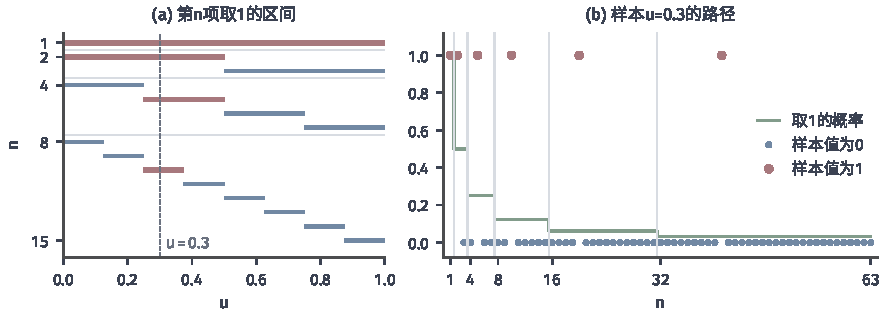
\includegraphics[width=150mm]{figures/02-abstract-mathematics/02-probability-spaces/matplotlib/conv-dyadic-sweep/figure.pdf}
  \caption{二进区间扫描$X_n=\mathbb I_{\{U\in[j/2^k,(j+1)/2^k)\}}$，$n=2^k+j$。(a) 前$15$项各自取$1$的区间，浅色横线分隔不同轮次，红色标出包含$u=0.3$的区间；(b) 样本$u=0.3$的路径$X_n(0.3)$，$n\leq63$（红点为$1$，蓝点为$0$），绿色阶梯为$\mathbb P(X_n=1)=2^{-k}$，竖线标出每一轮的起点$n=2^k$。}
  \label{fig:conv-dyadic-sweep}
\end{figure*}

\subsection{$p$阶平均收敛}

\paragraph{误差幅度的平均}
依概率收敛只问误差是否超过阈值，不问超过多少。
如果大误差虽然少见，一旦出现却非常大，我们往往希望把幅度也计入考虑，这就要对误差取平均。

\begin{definition}[$p$阶平均收敛]
\label{def:conv-mean}
设$1\leq p<\infty$，$\mathbb E|X_n|^p<\infty$对每个$n$成立，且$\mathbb E|X|^p<\infty$。若
\[
  \lim_{n\to\infty}\mathbb E|X_n-X|^p=0,
\]
则称$X_n$\term{$p$阶平均收敛}（convergence in $p$-th mean）于$X$，记作$X_n\xrightarrow{L^p}X$。
\end{definition}

记号$\xrightarrow{L^p}$只是“$\mathbb E|X_n-X|^p\to0$”的简写，本章不使用$L^p$作为函数空间的范数、完备性等结构，那些内容属于第~\ref{part:function-spaces}部分。
两个有限$p$阶矩的随机变量之差仍有有限$p$阶矩，因为$|a-b|^p\leq2^{p-1}(|a|^p+|b|^p)$（函数$t\mapsto t^p$在$[0,\infty)$上凸）。
$p=1$时$\mathbb E|X_n-X|$是平均绝对误差；$p=2$时$\mathbb E(X_n-X)^2$是均方误差，相应的收敛也叫\term{均方收敛}（mean-square convergence）。
$p$越大，大误差在平均中所占的分量越重：误差为$10$的事件在$p=1$时贡献$10$倍概率，在$p=2$时贡献$100$倍概率。

回到二进区间扫描。$X_n$只取$0$和$1$，所以对任意$p\geq1$，$\mathbb E|X_n|^p=\mathbb P(X_n=1)=2^{-k}\to0$，即$X_n\xrightarrow{L^p}0$。
这个例子在每一种平均意义下都收敛，却没有一个样本结果收敛。

\paragraph{有限维随机向量}
对取值于$\mathbb R^d$的随机向量$\bm X_n=(X_{n,1},\ldots,X_{n,d})$与$\bm X$，用欧氏范数代替绝对值：$\bm X_n\xrightarrow{L^p}\bm X$指$\mathbb E\lVert\bm X_n-\bm X\rVert_2^p\to0$。
它与逐坐标的$p$阶平均收敛等价。
记$\bm x\in\mathbb R^d$的坐标为$x_i$。一方面$|x_i|\leq\lVert\bm x\rVert_2$；另一方面
\[
  \lVert\bm x\rVert_2^p\leq\bigl(d\max_i|x_i|^2\bigr)^{p/2}=d^{p/2}\max_i|x_i|^p\leq d^{p/2}\sum_{i=1}^d|x_i|^p.
\]
把$\bm x=\bm X_n-\bm X$代入并取期望，得到
\[
  \mathbb E|X_{n,i}-X_i|^p\leq\mathbb E\lVert\bm X_n-\bm X\rVert_2^p\leq d^{p/2}\sum_{i=1}^d\mathbb E|X_{n,i}-X_i|^p,
\]
左式说明向量收敛蕴含每个坐标收敛，右式说明$d$个坐标都收敛时向量也收敛。
同样的两个不等式也说明，向量的几乎处处收敛和依概率收敛都与逐坐标的相应收敛等价；对依概率收敛，只需注意$\{\lVert\bm X_n-\bm X\rVert_2>\varepsilon\}\subseteq\bigcup_i\{|X_{n,i}-X_i|>\varepsilon/\sqrt d\}$。
这里只用到有限维的范数比较，维数$d$固定是关键：常数$d^{p/2}$随维数增大，无限维时不能照搬。
下文因此只对实值随机变量叙述结论。

\subsection{蕴含关系与反例}

\paragraph{三条蕴含与极限的唯一性}
有了三种定义，自然要问它们之间谁强谁弱。
下面的定理汇总能直接证明的蕴含关系。

\begin{theorem}[收敛方式之间的蕴含]
\label{thm:conv-implications}
设$X_n,X$是$(\Omega,\mathcal F,\mathbb P)$上的随机变量。
\begin{enumerate}
  \item 若$X_n\xrightarrow{\mathrm{a.s.}}X$，则$X_n\xrightarrow{\mathbb P}X$。
  \item 若对某个$1\leq p<\infty$有$X_n\xrightarrow{L^p}X$，则$X_n\xrightarrow{\mathbb P}X$。
  \item 若$1\leq p<q<\infty$且$X_n\xrightarrow{L^q}X$，则$X_n\xrightarrow{L^p}X$。
  \item 若$X_n\xrightarrow{\mathbb P}X$且$X_n\xrightarrow{\mathbb P}X'$，则$X=X'$几乎必然成立。
\end{enumerate}
\end{theorem}

\begin{proof}
(1) 固定$\varepsilon>0$。在使$X_n(\omega)\to X(\omega)$的概率为$1$的事件上，$\mathbb I_{\{|X_n-X|>\varepsilon\}}(\omega)$从某一项起恒为$0$，所以这些示性函数几乎处处趋于$0$；它们都以常数$1$为界，而常数$1$在概率测度下可积。
由控制收敛定理（定理~\ref{thm:integral-dominated-convergence}；常数控制的特例常称有界收敛定理），$\mathbb P(|X_n-X|>\varepsilon)=\mathbb E\,\mathbb I_{\{|X_n-X|>\varepsilon\}}\to0$。

(2) 第~\ref{chap:probability-models}章定理~\ref{thm:pmod-markov}的Markov不等式说，非负随机变量$Y$满足$\mathbb P(Y\geq t)\leq\mathbb EY/t$，$t>0$。取$Y=|X_n-X|^p$，$t=\varepsilon^p$，得
\[
  \mathbb P(|X_n-X|>\varepsilon)\leq\mathbb P(|X_n-X|^p\geq\varepsilon^p)\leq\frac{\mathbb E|X_n-X|^p}{\varepsilon^p}\to0.
\]

(3) 由第~\ref{chap:probability-models}章定理~\ref{thm:pmod-moment-monotone}，有限$q$阶矩蕴含有限$p$阶矩，所以$\mathbb E|X_n-X|^p$有定义。
令$Y=|X_n-X|^p\geq0$，函数$\varphi(t)=t^{q/p}$在$[0,\infty)$上凸，由定理~\ref{thm:pmod-jensen}的Jensen不等式$\varphi(\mathbb EY)\leq\mathbb E\varphi(Y)$，
\[
  \bigl(\mathbb E|X_n-X|^p\bigr)^{q/p}\leq\mathbb E|X_n-X|^q\to0.
\]

(4) 由三角不等式，$|X-X'|>2\varepsilon$时$|X_n-X|>\varepsilon$与$|X_n-X'|>\varepsilon$至少有一个成立，所以对每个$n$，
\[
  \mathbb P(|X-X'|>2\varepsilon)\leq\mathbb P(|X_n-X|>\varepsilon)+\mathbb P(|X_n-X'|>\varepsilon).
\]
左侧与$n$无关，右侧趋于$0$，故$\mathbb P(|X-X'|>2\varepsilon)=0$。
取$\varepsilon=1/m$，$\{X\neq X'\}=\bigcup_m\{|X-X'|>2/m\}$是可数个零概率事件的并，概率为$0$。
\end{proof}

结论(3)用到了$\mathbb P$是概率测度：Jensen不等式是对总质量为$1$的测度取平均才成立的，在Lebesgue测度这样的无穷测度上，$q$阶积分小并不能推出$p$阶积分小。
结论(3)的方向也不能颠倒，下文用尖峰的变形说明低阶平均收敛推不出高阶平均收敛。
结论(4)说明依概率极限在几乎必然相等的意义下唯一；由(1)和(2)，几乎处处极限与$p$阶平均极限也同样唯一，三种收敛若同时成立，极限必定一致。

\paragraph{两类反例}
上述蕴含能否反过来？
二进区间扫描已经回答了一半：它依概率收敛，也在每个$p$阶平均意义下收敛，却不几乎处处收敛。
所以依概率收敛和平均收敛都不能推出几乎处处收敛。
另一半需要一个方向相反的例子：误差几乎处处趋于零，平均误差却不趋于零。

\begin{example}[尖峰]
\label{ex:conv-spike}
取$U\sim\mathrm{Unif}[0,1)$，令$X_n=n\,\mathbb I_{\{0<U<1/n\}}$。
对每个$u\in(0,1)$，只要$n>1/u$就有$X_n(u)=0$；$u=0$时所有$X_n(0)=0$。所以每个样本结果上都有$X_n\to0$，$X_n\xrightarrow{\mathrm{a.s.}}0$。
但
\[
  \mathbb E|X_n|=n\cdot\mathbb P(0<U<1/n)=n\cdot\frac1n=1,
\]
平均误差恒为$1$，不趋于$0$；$p>1$时的平均误差$\mathbb E|X_n|^p=n^{p-1}$甚至趋于无穷。
\end{example}

图~\ref{fig:conv-spike}显示了尖峰的机制：$X_n$在越来越窄的区间$(0,1/n)$上取越来越大的值$n$，每个函数图像下的面积都是$1$。
样本$u=0.3$只在$n=1,2,3$处取到非零值，此后永远为$0$；取非零值的概率是$1/n$，也趋于零。
期望由面积决定，而面积从未减少，它只是被挤进了一个越来越小的事件里。

\begin{figure*}[htbp]
  \centering
  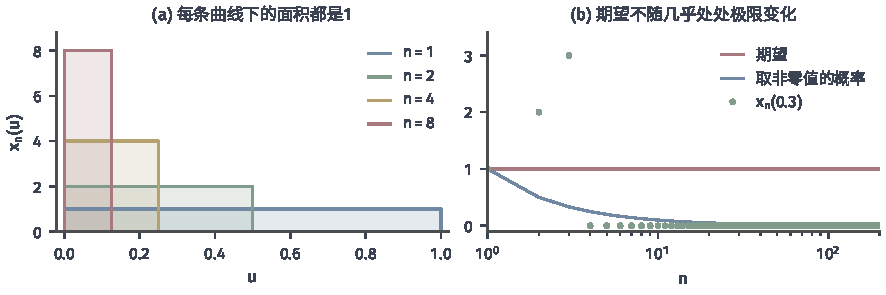
\includegraphics[width=150mm]{figures/02-abstract-mathematics/02-probability-spaces/matplotlib/conv-spike/figure.pdf}
  \caption{尖峰$X_n=n\,\mathbb I_{\{0<U<1/n\}}$，$U\sim\mathrm{Unif}[0,1)$。(a) 函数$x_n(u)=n\,\mathbb I_{(0,1/n)}(u)$在$n=1,2,4,8$时的图像，阴影面积均为$1$；(b) 横轴为对数刻度：$\mathbb E|X_n|$恒为$1$（红线），$\mathbb P(X_n\neq0)=1/n$（蓝线），绿点为样本$u=0.3$处的取值，$n\geq4$时均为$0$。}
  \label{fig:conv-spike}
\end{figure*}

两类例子分别暴露了两种不同的“坏”。
二进区间扫描中，误差每次出现时幅度都是$1$，但它反复出现，没有一条样本路径能摆脱它；尖峰中误差对每条路径只出现有限次，但出现时幅度极大，足以把平均误差维持在固定水平。
尖峰还满足$\mathbb P(|X_n|>\varepsilon)\leq1/n\to0$，所以它同时说明依概率收敛推不出一阶平均收敛。
类似地，取$1\leq p<q$，令$X_n=n^{1/q}\,\mathbb I_{\{0<U<1/n\}}$，则$\mathbb E|X_n|^p=n^{p/q-1}\to0$，而$\mathbb E|X_n|^q=1$，所以$p$阶平均收敛推不出$q$阶平均收敛。

图~\ref{fig:conv-implications}汇总了本节已证明的蕴含和三个反例。
图中没有单独画出的反向关系，可以由箭头与上面的例子组合判断。
例如，若依概率收敛蕴含$p$阶平均收敛，接在“几乎处处收敛蕴含依概率收敛”之后，就会得到几乎处处收敛蕴含$p$阶平均收敛，与尖峰矛盾；$p$阶平均收敛不能推出几乎处处收敛，则直接由二进区间扫描看出，因为它在每个$p$阶平均意义下都收敛，却没有一个样本结果收敛。
下两节的任务，是找出在什么附加条件下图中的虚线可以改成实线：第~\ref{sec:conv-events}节处理从依概率到几乎处处的方向，第~\ref{sec:conv-expectation-limits}节处理从几乎处处或依概率到平均收敛的方向。

\begin{figure*}[htbp]
  \centering
  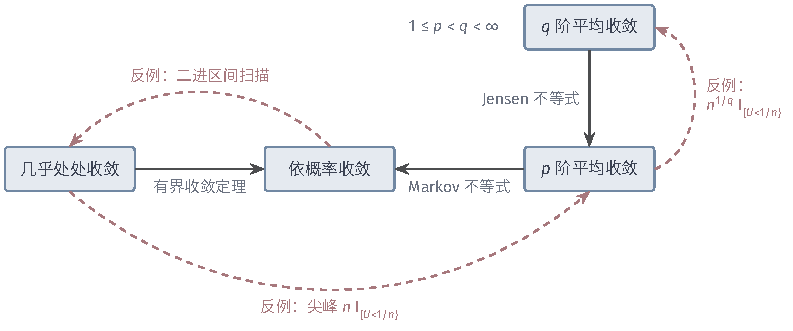
\includegraphics[width=134mm]{figures/02-abstract-mathematics/02-probability-spaces/tikz/conv-implications/figure.pdf}
  \caption{三种收敛方式的关系，$1\leq p<q<\infty$。黑色实线是定理~\ref{thm:conv-implications}证明的蕴含，旁注所用工具；红色虚线表示该方向的蕴含不成立，旁注反例，$U\sim\mathrm{Unif}[0,1)$。}
  \label{fig:conv-implications}
\end{figure*}

\section{事件列与收敛判据}
\label{sec:conv-events}

上一节的两类反例可以翻译成一个关于集合的问题：误差超过阈值的事件，是否发生无穷多次。
二进区间扫描中，每个样本结果都无穷多次落入坏事件；尖峰中，每个样本结果只落入有限次。
本节先给“无穷多次发生”和“最终总是发生”以精确的集合表示，再用概率的求和判断它们的概率，由此得到依概率收敛与几乎处处收敛之间的桥梁——子列判据；最后补充独立序列的尾事件只能取概率$0$或$1$的性质。

\subsection{事件的上极限与下极限}

\paragraph{无穷多次与最终总是}
设$A_1,A_2,\ldots$是一列事件。
说样本结果$\omega$属于“无穷多个$A_n$”，就是说无论走到多晚的位置$m$，后面总还有某个$n\geq m$使$\omega\in A_n$；
说$\omega$“最终总在$A_n$中”，就是说存在某个位置$m$，此后每个$n\geq m$都有$\omega\in A_n$。
把“对所有$m$”写成交、“存在$m$”写成并，得到如下定义。

\begin{definition}[事件列的上极限与下极限]
\label{def:conv-limsup-events}
事件列$(A_n)$的\term{上极限}（limit superior）与\term{下极限}（limit inferior）分别为
\[
  \limsup_{n\to\infty}A_n=\bigcap_{m=1}^{\infty}\bigcup_{n\geq m}A_n,\qquad
  \liminf_{n\to\infty}A_n=\bigcup_{m=1}^{\infty}\bigcap_{n\geq m}A_n.
\]
\end{definition}

两者的区别只在量词的顺序。
上极限先对每个$m$取“后面某一项”，再要求对所有$m$成立，所以$\omega\in\limsup_nA_n$当且仅当$\omega$属于无穷多个$A_n$，常写作$\{A_n\ \text{i.o.}\}$（infinitely often）。
下极限先固定某个$m$，再要求“后面每一项”，所以$\omega\in\liminf_nA_n$当且仅当$\omega$从某一项起属于所有$A_n$。
最终总在的样本结果当然也无穷多次出现，故$\liminf_nA_n\subseteq\limsup_nA_n$。
取补集时并与交互换，得到$(\limsup_nA_n)^c=\liminf_nA_n^c$：不属于无穷多个$A_n$，等价于最终总不属于$A_n$。
两者都由可数次交、并得到，所以都是事件。

图~\ref{fig:conv-limsup-liminf}用三个样本结果说明这两个集合。
$\omega_1$在所有偶数项中出现，次数无穷但始终有缺口，它属于上极限而不属于下极限；$\omega_2$在第$7$项之后不再出现，两者都不属于；$\omega_3$从第$8$项起每项都出现，属于下极限，也就属于上极限。
图中只能画出有限多列，判断依据是右侧所写的延续规律，而不是前$16$列。

\begin{figure*}[htbp]
  \centering
  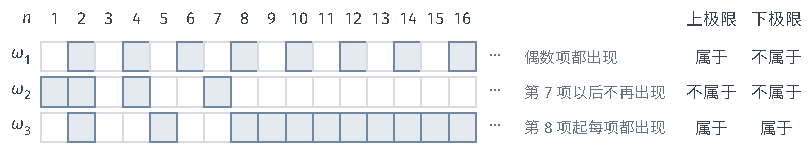
\includegraphics[width=138mm]{figures/02-abstract-mathematics/02-probability-spaces/tikz/conv-limsup-liminf/figure.pdf}
  \caption{事件列的上极限与下极限示意。第$\omega$行第$n$列的阴影格表示$\omega\in A_n$；三个样本结果的归属按右侧所写规律无限延续，最右两列给出它们是否属于$\limsup_nA_n$与$\liminf_nA_n$。}
  \label{fig:conv-limsup-liminf}
\end{figure*}

\paragraph{收敛与坏事件只发生有限次}
把坏事件代入上极限，就得到几乎处处收敛的事件刻画。
对$\varepsilon>0$，记$A_n(\varepsilon)=\{|X_n-X|>\varepsilon\}$。
数列$X_n(\omega)$收敛到$X(\omega)$，当且仅当对每个$\varepsilon>0$，$\omega$只属于有限多个$A_n(\varepsilon)$。
由于$A_n(\varepsilon)$随$\varepsilon$减小而增大，只需检查$\varepsilon=1/m$，于是
\[
  \{X_n\not\to X\}=\bigcup_{m=1}^{\infty}\limsup_{n\to\infty}A_n(1/m).
\]
这是式~\eqref{eq:conv-convergence-event}取补集后的形式。右侧是可数并，所以下面的判据成立。

\begin{lemma}[几乎处处收敛的事件判据]
\label{lem:conv-as-criterion}
$X_n\xrightarrow{\mathrm{a.s.}}X$，当且仅当对每个$\varepsilon>0$都有$\mathbb P\bigl(\limsup_nA_n(\varepsilon)\bigr)=0$。
\end{lemma}

\begin{proof}
若$X_n\xrightarrow{\mathrm{a.s.}}X$，每个$\limsup_nA_n(\varepsilon)$都包含于零概率事件$\{X_n\not\to X\}$。
反之，若每个$\limsup_nA_n(1/m)$概率为零，它们的可数并$\{X_n\not\to X\}$概率也为零。
\end{proof}

与依概率收敛比较，后者要求的是$\mathbb P(A_n(\varepsilon))\to0$。
由概率的连续性，$\bigcup_{n\geq m}A_n$随$m$递减到$\limsup_nA_n$，而每个$\bigcup_{n\geq m}A_n$的概率不小于其中任一$A_n$的概率，所以
\[
  \mathbb P\Bigl(\limsup_{n\to\infty}A_n\Bigr)=\lim_{m\to\infty}\mathbb P\Bigl(\bigcup_{n\geq m}A_n\Bigr)\geq\limsup_{n\to\infty}\mathbb P(A_n).
\]
这个不等式只给出上极限概率的下界。当单项概率$\mathbb P(A_n)$趋于$0$时，下界是$0$，它对上极限的概率没有提供任何信息。
二进区间扫描正是如此：$\mathbb P(A_n(1/2))=2^{-k}\to0$，但每个样本结果都无穷多次落入$A_n(1/2)$，$\limsup_nA_n(1/2)=\Omega$。
要从单项概率推出上极限的概率，需要更多信息，下一小节给出两种情形。

\subsection{Borel--Cantelli引理}

\paragraph{可求和的概率}
如果坏事件的概率不仅趋于零，而且总和有限，那么一个样本结果落入的坏事件个数平均起来是有限的，直觉上它就不应落入无穷多个。
下面的引理同时给出这一方向与它在独立条件下的反面。

\begin{lemma}[Borel--Cantelli引理]
\label{lem:conv-borel-cantelli}
设$A_1,A_2,\ldots$是事件。
\begin{enumerate}
  \item 若$\sum_{n=1}^{\infty}\mathbb P(A_n)<\infty$，则$\mathbb P(\limsup_nA_n)=0$。
  \item 若$A_1,A_2,\ldots$相互独立且$\sum_{n=1}^{\infty}\mathbb P(A_n)=\infty$，则$\mathbb P(\limsup_nA_n)=1$。
\end{enumerate}
\end{lemma}

这两条结论合称\term{Borel--Cantelli引理}。第一部分对任意事件列成立，不需要任何独立性。

\begin{proof}[第一部分的证明]
对每个$m$，$\limsup_nA_n\subseteq\bigcup_{n\geq m}A_n$。由概率的可数次可加性，
\[
  \mathbb P\Bigl(\limsup_{n\to\infty}A_n\Bigr)\leq\mathbb P\Bigl(\bigcup_{n\geq m}A_n\Bigr)\leq\sum_{n\geq m}\mathbb P(A_n).
\]
右侧是收敛级数的尾和，随$m\to\infty$趋于$0$；左侧与$m$无关，所以等于$0$。
\end{proof}

这个证明还可以从“发生次数”的角度理解。
令$N=\sum_n\mathbb I_{A_n}$为发生的事件个数，由单调收敛定理$\mathbb EN=\sum_n\mathbb P(A_n)<\infty$，所以$N$几乎必然有限，这正是$\mathbb P(\limsup_nA_n)=0$。
结合引理~\ref{lem:conv-as-criterion}，第一部分给出一个常用的充分条件：若对每个$\varepsilon>0$都有$\sum_n\mathbb P(|X_n-X|>\varepsilon)<\infty$，则$X_n\xrightarrow{\mathrm{a.s.}}X$。
它把逐项的误差概率转化为逐样本最终成立的结论，代价是要求概率可求和，而不只是趋于零。

\paragraph{独立且概率和发散的情形}
第二部分说的是另一个方向：若事件之间没有相互牵制，概率和发散就足以保证无穷多次发生。

\begin{proof}[第二部分的证明]
只需证明对每个$m$，$\mathbb P(\bigcap_{n\geq m}A_n^c)=0$，因为$(\limsup_nA_n)^c=\bigcup_m\bigcap_{n\geq m}A_n^c$是可数个这样的事件之并。
固定$m<M$。由于$A_n$相互独立，它们的补事件也相互独立（第~\ref{chap:probability-models}章定理~\ref{thm:pmod-independence-grouping}：对独立事件生成的$\sigma$代数取元素，独立性保持），于是
\[
  \mathbb P\Bigl(\bigcap_{n=m}^MA_n^c\Bigr)=\prod_{n=m}^M\bigl(1-\mathbb P(A_n)\bigr)\leq\prod_{n=m}^Me^{-\mathbb P(A_n)}=\exp\Bigl(-\sum_{n=m}^M\mathbb P(A_n)\Bigr),
\]
这里用了$1-x\leq e^{-x}$。
令$M\to\infty$，左侧事件递减到$\bigcap_{n\geq m}A_n^c$，由概率的连续性左侧趋于$\mathbb P(\bigcap_{n\geq m}A_n^c)$；右侧因级数发散而趋于$0$。
\end{proof}

独立性在这里不能省去。
取一个满足$\mathbb P(A)=1/2$的事件$A$，令所有$A_n=A$，则$\sum_n\mathbb P(A_n)=\infty$，但$\limsup_nA_n=A$，概率只有$1/2$：这些事件完全相同，一个样本结果要么一次也不落入，要么每次都落入。
二进区间扫描中同一轮的事件互不相交，也不独立，但它们恰好覆盖整个样本空间，所以$\limsup$也是全集；那里的结论来自区间覆盖的几何事实，而不是第二部分。

图~\ref{fig:conv-borel-cantelli}用模拟对照了两种情形。
两组事件都相互独立，左图$\mathbb P(A_n)=1/n^2$，右图$\mathbb P(A_n)=1/n$。
左图中每条路径在开始时跳几次就停下来，发生总次数的期望是$\sum_n1/n^2=\pi^2/6\approx1.64$；右图中路径一直在上升，期望次数$\sum_{k\leq n}1/k$约为$\ln n$，虽然增长很慢，却没有上限。

\begin{figure*}[htbp]
  \centering
  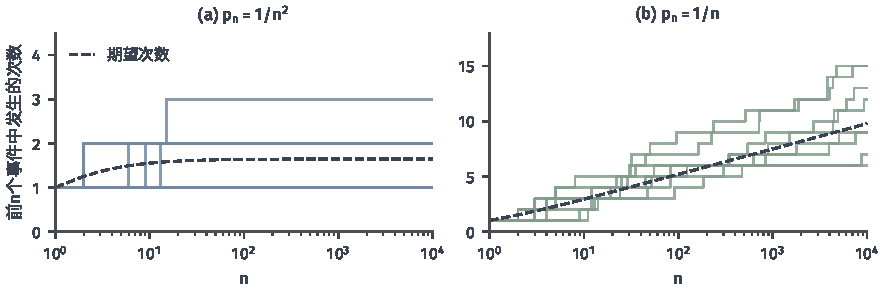
\includegraphics[width=150mm]{figures/02-abstract-mathematics/02-probability-spaces/matplotlib/conv-borel-cantelli/figure.pdf}
  \caption{独立事件发生次数的模拟，横轴为对数刻度。每个面板用固定随机种子画出$8$条路径，纵轴为$A_1,\ldots,A_n$中发生的个数，虚线为其期望$\sum_{k\leq n}\mathbb P(A_k)$。(a) $\mathbb P(A_n)=1/n^2$，各路径在$n=10^4$时的次数为$1$到$3$；(b) $\mathbb P(A_n)=1/n$，次数为$6$到$15$且仍在增长。}
  \label{fig:conv-borel-cantelli}
\end{figure*}

\subsection{依概率收敛的子列判据}

\paragraph{抽取几乎处处收敛的子列}
二进区间扫描整列不几乎处处收敛，但如果只看一部分项呢？
取$n_k=2^k$，即每一轮的第一项，$X_{2^k}=\mathbb I_{\{U<2^{-k}\}}$。
对每个$u>0$，一旦$2^{-k}\leq u$，此后这个子列就恒为$0$；所以这个子列几乎处处收敛到$0$。
关键在于：这个子列的坏事件概率$2^{-k}$可求和，而整列的坏事件概率在每一轮中加起来都是$1$，总和发散。
这启发我们，从任何依概率收敛的序列中，都可以挑出坏事件概率可求和的一个子列，再用Borel--Cantelli引理。

\begin{theorem}[依概率收敛的子列判据]
\label{thm:conv-subsequence}
$X_n\xrightarrow{\mathbb P}X$，当且仅当$(X_n)$的每个子列$(X_{n_j})$都有进一步的子列$(X_{n_{j_k}})$满足$X_{n_{j_k}}\xrightarrow{\mathrm{a.s.}}X$。
特别地，若$X_n\xrightarrow{\mathbb P}X$，则存在子列$X_{n_k}\xrightarrow{\mathrm{a.s.}}X$。
\end{theorem}

\begin{proof}[必要性]
设$X_n\xrightarrow{\mathbb P}X$，$(X_{n_j})$是任一子列，它同样依概率收敛于$X$。
对$k=1,2,\ldots$依次选取$j_k>j_{k-1}$，使
\[
  \mathbb P\bigl(|X_{n_{j_k}}-X|>2^{-k}\bigr)\leq2^{-k};
\]
这是可以做到的，因为对固定的$k$，左侧的概率随$j\to\infty$趋于零。
记$B_k=\{|X_{n_{j_k}}-X|>2^{-k}\}$，则$\sum_k\mathbb P(B_k)\leq\sum_k2^{-k}=1<\infty$。
由引理~\ref{lem:conv-borel-cantelli}第一部分，几乎每个$\omega$只属于有限多个$B_k$，即存在依赖于$\omega$的$K$，使$k\geq K$时$|X_{n_{j_k}}(\omega)-X(\omega)|\leq2^{-k}$。
于是这些$\omega$上$X_{n_{j_k}}(\omega)\to X(\omega)$。
\end{proof}

证明中阈值和概率同时取$2^{-k}$。阈值趋于零保证最终误差变小；概率可求和保证坏事件只发生有限次。
图~\ref{fig:conv-subsequence}在二进区间扫描上显示了这一区别。
左图中，样本$u=0.3$的全序列每轮都有一个$1$，而方框标出的子列$n_k=2^k$在$k\geq2$后恒为$0$；右图比较两者坏事件概率的累计和，全序列每轮增加$1$，子列的累计和不超过$2$。
子列是事先确定的下标序列，不随$\omega$改变；对每一个这样选定的子列，Borel--Cantelli引理保证几乎所有样本结果最终都避开坏事件。

\begin{figure*}[htbp]
  \centering
  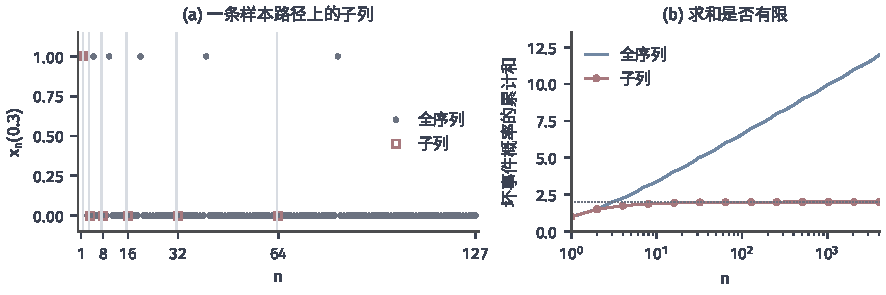
\includegraphics[width=150mm]{figures/02-abstract-mathematics/02-probability-spaces/matplotlib/conv-subsequence/figure.pdf}
  \caption{二进区间扫描中的子列抽取。(a) 样本$u=0.3$的全序列$X_n(0.3)$（灰点，$n\leq127$）与子列$n_k=2^k$（红色方框），竖线为各轮起点；(b) 坏事件概率$\mathbb P(X_n=1)$的累计和，横轴为对数刻度：全序列每轮增加$1$，到$n=2^{12}$约为$12$；子列$\sum_k2^{-k}$的累计和趋于$2$（点线）。}
  \label{fig:conv-subsequence}
\end{figure*}

\paragraph{充分性与反证}
反过来，如果每个子列都能再抽出几乎处处收敛到$X$的子列，原序列是否依概率收敛？

\begin{proof}[充分性]
若$X_n\xrightarrow{\mathbb P}X$不成立，则存在$\varepsilon>0$，使$\mathbb P(|X_n-X|>\varepsilon)$不趋于$0$；于是又存在$\delta>0$及子列$(n_j)$，使
\[
  \mathbb P\bigl(|X_{n_j}-X|>\varepsilon\bigr)\geq\delta\quad\text{对所有}j\text{成立}.
\]
按假设，$(X_{n_j})$有进一步的子列$X_{n_{j_k}}\xrightarrow{\mathrm{a.s.}}X$；由定理~\ref{thm:conv-implications}(1)，它也依概率收敛于$X$，故$\mathbb P(|X_{n_{j_k}}-X|>\varepsilon)\to0$，与上式中的下界$\delta$矛盾。
\end{proof}

判据要求的是“每个子列”都有进一步的子列收敛到\emph{同一个}$X$，只找到一个收敛子列是不够的。
令$X_n=0$（$n$为奇数），$X_n=1$（$n$为偶数），即在$0$与$1$之间交替的常数随机变量。
偶数项组成的子列收敛到$1$，奇数项组成的子列收敛到$0$；若$X_n\xrightarrow{\mathbb P}X$，两个子列也都依概率收敛于$X$，由极限唯一性$X$几乎必然既等于$1$又等于$0$，矛盾。所以这一列不依概率收敛。

子列判据的用处，是让依概率收敛可以借用那些需要几乎处处收敛作条件的定理。
例如，设$g:\mathbb R\to\mathbb R$连续，$X_n\xrightarrow{\mathbb P}X$。
任取子列，先抽出进一步的子列几乎处处收敛于$X$，由$g$的连续性，这个子列上$g(X_{n_{j_k}})\to g(X)$几乎处处成立；由判据的充分性，$g(X_n)\xrightarrow{\mathbb P}g(X)$。
下一节将以同样方式把控制收敛定理推广到依概率收敛。

\subsection{尾事件与零一律（补充）}

本小节补充独立序列的尾事件性质。
前面的子列判据和后面强大数律的证明都不依赖这里的结论，读者可以先跳过；但它解释了一个在后文反复出现的现象：随机级数是否收敛、样本平均是否收敛，这类问题的答案在独立情形下总是“几乎必然是”或“几乎必然不是”。

\paragraph{尾$\sigma$代数}
考察一列随机变量$X_1,X_2,\ldots$。
有些事件不受前面任何有限多项的影响。
例如级数$\sum_nX_n$是否收敛：去掉或改动前$m-1$项，部分和只差一个固定的有限数，收敛与否不变，所以这个事件可以只用$X_m,X_{m+1},\ldots$来判断。
又如样本平均$\bar X_n=\frac1n\sum_{k=1}^nX_k$是否收敛到给定常数$c$：由于$\frac1n\sum_{k<m}X_k\to0$对每个样本结果成立，$\bar X_n\to c$当且仅当$\frac1n\sum_{k=m}^nX_k\to c$，后者也只依赖$X_m,X_{m+1},\ldots$。
相反，“级数的和等于$1$”就不是这样的事件，因为改动$X_1$会改变和的值。

用$\sigma(X_m,X_{m+1},\ldots)$表示由$X_m,X_{m+1},\ldots$生成的$\sigma$代数，即使这些随机变量都可测的最小$\sigma$代数（第~\ref{chap:probability-models}章定义~\ref{def:pmod-generated-sigma}的推广）。

\begin{definition}[尾$\sigma$代数]
\label{def:conv-tail-sigma}
随机变量列$(X_n)$的\term{尾$\sigma$代数}（tail sigma-algebra）为
\[
  \mathcal T=\bigcap_{m=1}^{\infty}\sigma(X_m,X_{m+1},\ldots),
\]
其中的事件称为\term{尾事件}（tail event）。
\end{definition}

上面两个例子中的事件对每个$m$都属于$\sigma(X_m,X_{m+1},\ldots)$：用式~\eqref{eq:conv-convergence-event}的写法把“收敛”展开为可数次交并，每一步只用到下标不小于$m$的变量。所以它们都是尾事件。

\paragraph{Kolmogorov零一律}
尾事件不受任何有限个初始变量影响。若各变量相互独立，尾事件就与任何有限个初始变量独立；而尾事件本身又由全部变量决定，下面的证明说明这迫使它与自己独立，即$\mathbb P(A)=\mathbb P(A)^2$。

\begin{theorem}[Kolmogorov零一律]
\label{thm:conv-zero-one}
设$X_1,X_2,\ldots$相互独立，$\mathcal T$是它们的尾$\sigma$代数，则每个$A\in\mathcal T$都满足$\mathbb P(A)=0$或$\mathbb P(A)=1$。
\end{theorem}

这一结论称为\term{Kolmogorov零一律}（Kolmogorov zero-one law）。证明的思路是把尾事件与越来越长的初始段比较。

\begin{proof}
记$\mathcal F_n=\sigma(X_1,\ldots,X_n)$。
按第~\ref{chap:probability-models}章定理~\ref{thm:pmod-independence-grouping}，独立变量分成不相交的两组后，两组生成的$\sigma$代数仍独立，所以$\mathcal F_n$与$\sigma(X_{n+1},X_{n+2},\ldots)$独立；$\mathcal T$包含于后者，故$\mathcal F_n$与$\mathcal T$独立。

固定$A\in\mathcal T$。在$\mathcal F_\infty=\sigma(X_1,X_2,\ldots)$上定义两个有限测度$\mu(B)=\mathbb P(B\cap A)$与$\nu(B)=\mathbb P(B)\mathbb P(A)$。
集合族$\mathcal C=\bigcup_n\mathcal F_n$包含$\Omega$，对有限交封闭（$\mathcal F_n$递增，两个集合总落在同一个$\mathcal F_n$中），并生成$\mathcal F_\infty$；上一段说明$\mu=\nu$在$\mathcal C$上成立。
由第~\ref{chap:measures}章定理~\ref{thm:measure-uniqueness}，$\mu=\nu$在整个$\mathcal F_\infty$上成立。
$A$本身属于$\mathcal T\subseteq\mathcal F_\infty$，取$B=A$得$\mathbb P(A)=\mathbb P(A)^2$，所以$\mathbb P(A)\in\{0,1\}$。
\end{proof}

于是对独立的$X_n$，随机级数$\sum_nX_n$几乎必然收敛或几乎必然发散，样本平均几乎必然收敛到$c$或几乎必然不收敛到$c$，没有中间情形。
零一律只说概率是$0$或$1$，并不告诉我们是哪一个。
要判断某个随机级数确实收敛，仍需要第~\ref{sec:conv-partial-sums}节的方差估计；要判断样本平均确实收敛到均值，仍需要第~\ref{sec:conv-sample-means}节的证明。
所以零一律不能代替强大数律的证明，它的作用是说明那里得到的“几乎必然”结论不是偶然的。

\section{随机变量列的期望极限}
\label{sec:conv-expectation-limits}

本节研究$X_n$趋于$X$之后，期望$\mathbb EX_n$是否趋于$\mathbb EX$，以及平均误差$\mathbb E|X_n-X|^p$是否趋于零。
这里的期望是对底层概率测度$\mathbb P$的积分：固定$n$时，$\mathbb EX_n$是一个确定的数，而不是把前$n$个观测相加再除以$n$得到的样本平均，后者是第~\ref{sec:conv-sample-means}节的对象。
尖峰例子已经表明，几乎处处收敛本身不足以让极限进入期望。
我们先用已有的可积控制条件处理这个问题，并借助子列判据把它推广到依概率收敛；再从尖峰的失效机制中提炼出一致可积，最后证明它恰好刻画了依概率收敛何时升级为一阶平均收敛。

\subsection{有界与可积控制下的期望极限}

\paragraph{共同的可积上界}
尖峰缺少的是什么？
若存在一个随机变量$Y$同时控制所有$X_n=n\,\mathbb I_{\{0<U<1/n\}}$，它在$U=u\in(0,1)$处至少要达到$\sup_nX_n(u)$，即小于$1/u$的最大正整数，这个数不小于$1/u-1$；而$\mathbb E(1/U)=\int_0^1u^{-1}\,du=\infty$。
所以尖峰没有可积的共同上界，越来越高的峰合起来的“包络”面积是无穷大。

有了共同的可积上界，情况就不同了。
设$X_n\xrightarrow{\mathrm{a.s.}}X$，且存在$Y\geq0$，$\mathbb EY<\infty$，使每个$n$都有$|X_n|\leq Y$几乎必然成立。
可数个“$|X_n|\leq Y$”的例外事件与不收敛事件合并后仍是零概率事件，在其外取极限得$|X|\leq Y$，于是$|X_n-X|\leq2Y$。
对$|X_n-X|\to0$应用控制收敛定理（定理~\ref{thm:integral-dominated-convergence}），控制函数为$2Y$，得$\mathbb E|X_n-X|\to0$；再由
\[
  |\mathbb EX_n-\mathbb EX|=|\mathbb E(X_n-X)|\leq\mathbb E|X_n-X|
\]
得到$\mathbb EX_n\to\mathbb EX$。
$Y$取常数$c$时就是有界收敛：一列一致有界、几乎处处收敛的随机变量，其期望也收敛。
这里没有重新证明控制收敛定理，只是把它的条件翻译成概率语言：几乎处处收敛对应几乎处处的逐点收敛，共同上界对应可积控制函数。

\paragraph{依概率收敛下的控制收敛}
控制收敛定理要求逐点（几乎处处）收敛。
若只知道依概率收敛，就不能直接调用它；但子列判据允许我们先在子列上使用它，再回到整列。

\begin{theorem}[依概率收敛下的控制收敛]
\label{thm:conv-dominated-probability}
设$X_n\xrightarrow{\mathbb P}X$，且存在随机变量$Y\geq0$，$\mathbb EY<\infty$，使每个$n$都有$|X_n|\leq Y$几乎必然成立。
则$|X|\leq Y$几乎必然成立，$\mathbb E|X_n-X|\to0$，从而$\mathbb EX_n\to\mathbb EX$。
\end{theorem}

\begin{proof}
由定理~\ref{thm:conv-subsequence}，存在子列$X_{n_k}\xrightarrow{\mathrm{a.s.}}X$。在概率为$1$的事件上同时有$X_{n_k}\to X$与$|X_{n_k}|\leq Y$对所有$k$成立，取极限得$|X|\leq Y$几乎必然成立。

再证$\mathbb E|X_n-X|\to0$。若不然，存在$\delta>0$及子列$(n_j)$使$\mathbb E|X_{n_j}-X|\geq\delta$对所有$j$成立。
子列$(X_{n_j})$仍依概率收敛于$X$，再由定理~\ref{thm:conv-subsequence}抽出进一步的子列$X_{n_{j_k}}\xrightarrow{\mathrm{a.s.}}X$。
在这个子列上$|X_{n_{j_k}}-X|\leq2Y$几乎必然成立，由控制收敛定理$\mathbb E|X_{n_{j_k}}-X|\to0$，与下界$\delta$矛盾。
期望的收敛由$|\mathbb EX_n-\mathbb EX|\leq\mathbb E|X_n-X|$得到。
\end{proof}

证明中子列论证用了两次：一次得到极限的上界，一次把“整列不收敛”转化为“某个子列一直远离”，再与进一步子列上的控制收敛相矛盾。
依概率收敛本身不是控制收敛定理的条件；起作用的是子列判据提供的几乎处处收敛子列。

\begin{example}[有界函数的期望]
\label{ex:conv-bounded-function}
设估计量$\hat\theta_n\xrightarrow{\mathbb P}\theta$，$\theta$是常数，$g$是有界连续函数，$|g|\leq c$。
由上一节用子列判据得到的连续映射结论，$g(\hat\theta_n)\xrightarrow{\mathbb P}g(\theta)$；取$Y=c$，定理~\ref{thm:conv-dominated-probability}给出$\mathbb Eg(\hat\theta_n)\to g(\theta)$。
有界性不能去掉：令$\hat\theta_n=\theta+n\,\mathbb I_{\{0<U<1/n\}}$，取$g(t)=t$，则$\hat\theta_n\xrightarrow{\mathbb P}\theta$，但$\mathbb E\hat\theta_n=\theta+1$。
\end{example}

\subsection{一致可积的定义与判别}

\paragraph{尖峰把积分推向越来越小的事件}
共同的可积上界是充分条件，但要求太强。
例如对$n\geq3$令$X_n=\frac{n}{\ln n}\,\mathbb I_{\{0<U<1/n\}}$，它几乎处处趋于$0$，期望$1/\ln n$也趋于$0$；但$\sup_nX_n(u)$在$u$接近$0$时约为$\frac{1}{u\ln(1/u)}$，而$\int_0^{1/3}\frac{du}{u\ln(1/u)}=\infty$，所以它没有可积的共同上界。
这说明需要一个比共同上界更贴近问题的条件。

为此回到尖峰，找出它失效的确切原因。
对阈值$K\geq1$，$X_n=n\,\mathbb I_{\{0<U<1/n\}}$在$n\leq K$时从不超过$K$，在$n>K$时只要非零就超过$K$，所以
\[
  \mathbb E\bigl[X_n\,\mathbb I_{\{X_n>K\}}\bigr]=
  \begin{cases}0,&n\leq K,\\ 1,&n>K.\end{cases}
\]
对每个固定的$n$，这个尾部积分在$K\geq n$后变为$0$；但无论$K$多大，总有$n>K$的项把全部积分$1$放在阈值以上。
期望不随几乎处处极限变化，正是因为越来越小的事件仍携带固定大小的积分。
要排除这种现象，需要一个阈值同时控制整个序列的尾部积分。

\begin{definition}[一致可积]
\label{def:conv-uniform-integrability}
设$\{X_i:i\in I\}$是一族可积随机变量，$I$为任意指标集。若
\[
  \lim_{K\to\infty}\sup_{i\in I}\mathbb E\bigl[|X_i|\,\mathbb I_{\{|X_i|>K\}}\bigr]=0,
\]
则称这族随机变量\term{一致可积}（uniformly integrable）。
\end{definition}

“一致”指同一个$K$对全族有效。
单个可积随机变量$X$的尾部积分$\mathbb E[|X|\,\mathbb I_{\{|X|>K\}}]$随$K\to\infty$趋于$0$：被积函数几乎处处趋于$0$，且受$|X|$控制，由控制收敛定理即得。对有限族，上确界只是有限个趋于$0$的量取最大，所以有限族总是一致可积的。
尖峰说明可数族未必如此：每一项分别可积，尾部积分对每项分别趋于零，但上确界恒为$1$。

\paragraph{一致可积的判别}
直接验证定义往往不方便。下面的判别把一致可积与更容易检查的矩条件或控制条件联系起来。

\begin{theorem}[一致可积的判别]
\label{thm:conv-ui-criteria}
设$\{X_i:i\in I\}$是一族可积随机变量。
\begin{enumerate}
  \item 若这族一致可积，则$\sup_{i}\mathbb E|X_i|<\infty$。
  \item 若存在$Y\geq0$，$\mathbb EY<\infty$，使$|X_i|\leq Y$几乎必然对每个$i$成立，则这族一致可积。
  \item 若存在$r>1$使$C=\sup_i\mathbb E|X_i|^r<\infty$，则这族一致可积，且$\sup_i\mathbb E[|X_i|\,\mathbb I_{\{|X_i|>K\}}]\leq CK^{1-r}$。
  \item 若$A_i,B_i\geq0$，$0\leq W_i\leq A_i+B_i$，而$\{A_i\}$与$\{B_i\}$都一致可积，则$\{W_i\}$一致可积。
\end{enumerate}
\end{theorem}

\begin{proof}
(1) 取$K_0$使$\sup_i\mathbb E[|X_i|\,\mathbb I_{\{|X_i|>K_0\}}]\leq1$。把$|X_i|$按是否超过$K_0$拆开，
\[
  \mathbb E|X_i|=\mathbb E\bigl[|X_i|\,\mathbb I_{\{|X_i|\leq K_0\}}\bigr]+\mathbb E\bigl[|X_i|\,\mathbb I_{\{|X_i|>K_0\}}\bigr]\leq K_0+1.
\]

(2) $\{|X_i|>K\}\subseteq\{Y>K\}$且$|X_i|\leq Y$，所以$\mathbb E[|X_i|\,\mathbb I_{\{|X_i|>K\}}]\leq\mathbb E[Y\,\mathbb I_{\{Y>K\}}]$，右侧与$i$无关，且由单个可积变量的结论趋于$0$。

(3) 在事件$\{|X_i|>K\}$上，$|X_i|=|X_i|^r\cdot|X_i|^{1-r}\leq|X_i|^rK^{1-r}$，因为$1-r<0$。取期望得$\mathbb E[|X_i|\,\mathbb I_{\{|X_i|>K\}}]\leq K^{1-r}\mathbb E|X_i|^r\leq CK^{1-r}$。

(4) 在$\{A_i+B_i>K\}$上，$A_i,B_i$中较大者超过$K/2$，所以
\[
  W_i\,\mathbb I_{\{W_i>K\}}\leq(A_i+B_i)\,\mathbb I_{\{A_i+B_i>K\}}\leq2A_i\,\mathbb I_{\{A_i>K/2\}}+2B_i\,\mathbb I_{\{B_i>K/2\}},
\]
第一个不等号用了$W_i\leq A_i+B_i$与$\{W_i>K\}\subseteq\{A_i+B_i>K\}$。取期望再对$i$取上确界，右侧随$K\to\infty$趋于$0$。
\end{proof}

结论(1)的逆命题不成立：尖峰满足$\sup_n\mathbb E|X_n|=1$，却不一致可积。
一阶矩有界只限制了每项积分的总量，没有限制这份积分能被挤到多么稀有的事件上；结论(3)要求高于一阶的矩有界，正是对这种挤压的惩罚。
另一方面，一致可积也严格弱于结论(2)的共同控制。
前面没有可积上界的$X_n=\frac{n}{\ln n}\,\mathbb I_{\{0<U<1/n\}}$（$n\geq3$）在$X_n>K$时取值$n/\ln n$，尾部积分等于$\frac{n}{\ln n}\cdot\frac1n=\frac1{\ln n}$，否则为$0$；对$K\geq3$，$n/\ln n>K$迫使$n>K$，所以尾部积分的上确界不超过$1/\ln K\to0$，这族一致可积。

图~\ref{fig:conv-ui-tails}比较了两族随机变量。
尖峰族的尾部积分上确界对所有$K$都等于$1$；把峰高从$n$降为$\sqrt n$，得到$X_n=\sqrt n\,\mathbb I_{\{0<U<1/n\}}$，它满足$\mathbb EX_n^2=1$，由结论(3)取$r=2$，尾部积分上确界不超过$1/K$。
图中右栏显示尖峰族逐项的尾部积分：每条曲线在$K=n$处降到$0$，但$n$越大降得越晚，没有一个$K$能让所有曲线都降下来。

\begin{figure*}[htbp]
  \centering
  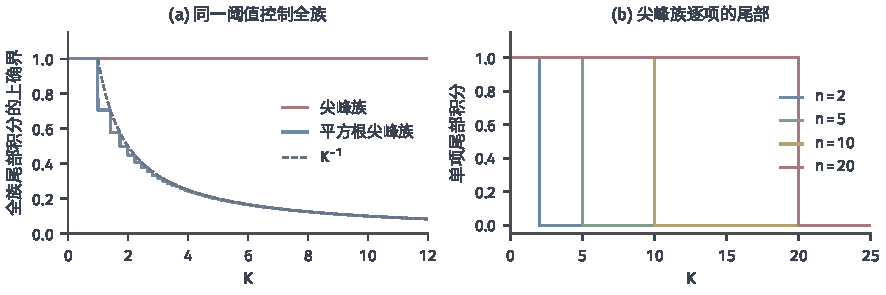
\includegraphics[width=150mm]{figures/02-abstract-mathematics/02-probability-spaces/matplotlib/conv-ui-tails/figure.pdf}
  \caption{尾部积分与一致可积，$U\sim\mathrm{Unif}[0,1)$。(a) $\sup_n\mathbb E[X_n\,\mathbb I_{\{X_n>K\}}]$随$K$的变化：尖峰族$X_n=n\,\mathbb I_{\{0<U<1/n\}}$恒为$1$；平方根尖峰族$X_n=\sqrt n\,\mathbb I_{\{0<U<1/n\}}$的精确值为$(\lfloor K^2\rfloor+1)^{-1/2}$，虚线为二阶矩给出的上界$1/K$。(b) 尖峰族中$n=2,5,10,20$各项的尾部积分$\mathbb E[X_n\,\mathbb I_{\{X_n>K\}}]=\mathbb I_{\{n>K\}}$。}
  \label{fig:conv-ui-tails}
\end{figure*}

\subsection{一致可积条件下的平均收敛}

\paragraph{一致可积与一阶平均收敛}
现在可以回答本节开头的问题：在依概率收敛的前提下，什么条件恰好保证平均误差趋于零？

\begin{theorem}[一致可积与一阶平均收敛]
\label{thm:conv-ui-l1}
设每个$X_n$可积，且$X_n\xrightarrow{\mathbb P}X$。则下列两条等价：
\begin{enumerate}
  \item $\{X_n\}$一致可积；
  \item $X$可积，且$\mathbb E|X_n-X|\to0$。
\end{enumerate}
此时$\mathbb EX_n\to\mathbb EX$。
\end{theorem}

\begin{proof}
(1)$\Rightarrow$(2)。先证$X$可积。取子列$X_{n_k}\xrightarrow{\mathrm{a.s.}}X$，由Fatou引理（引理~\ref{lem:integral-fatou}）与定理~\ref{thm:conv-ui-criteria}(1)，
\[
  \mathbb E|X|\leq\liminf_{k\to\infty}\mathbb E|X_{n_{k}}|\leq\sup_n\mathbb E|X_n|<\infty.
\]
再把误差分成有界部分和大值尾部。对$K>0$，令
\[
  \varphi_K(x)=\max\{-K,\min\{x,K\}\},
\]
它把$x$截到$[-K,K]$中，满足$|\varphi_K(x)-\varphi_K(y)|\leq|x-y|$与$|x-\varphi_K(x)|\leq|x|\,\mathbb I_{\{|x|>K\}}$。由三角不等式，
\[
  |X_n-X|\leq|\varphi_K(X_n)-\varphi_K(X)|+|X_n|\,\mathbb I_{\{|X_n|>K\}}+|X|\,\mathbb I_{\{|X|>K\}}.
\]
第一项满足$|\varphi_K(X_n)-\varphi_K(X)|\leq|X_n-X|$，所以$\varphi_K(X_n)\xrightarrow{\mathbb P}\varphi_K(X)$，且它们都以常数$K$为界；由定理~\ref{thm:conv-dominated-probability}，第一项的期望趋于$0$。于是
\[
  \limsup_{n\to\infty}\mathbb E|X_n-X|\leq\sup_n\mathbb E\bigl[|X_n|\,\mathbb I_{\{|X_n|>K\}}\bigr]+\mathbb E\bigl[|X|\,\mathbb I_{\{|X|>K\}}\bigr].
\]
左侧与$K$无关；令$K\to\infty$，右侧第一项由一致可积趋于$0$，第二项由$X$可积趋于$0$。

(2)$\Rightarrow$(1)。固定$\eta>0$，取$N$使$n>N$时$\mathbb E|X_n-X|<\eta$。
先看$n>N$的项。由$|X_n|\leq|X_n-X|+|X|$，
\[
  \mathbb E\bigl[|X_n|\,\mathbb I_{\{|X_n|>K\}}\bigr]\leq\mathbb E|X_n-X|+\mathbb E\bigl[|X|\,\mathbb I_{\{|X_n|>K\}}\bigr].
\]
对最后一项，按$|X|$是否超过另一个阈值$M$拆开，并用Markov不等式，
\[
  \begin{aligned}
  \mathbb E\bigl[|X|\,\mathbb I_{\{|X_n|>K\}}\bigr]
  &\leq\mathbb E\bigl[|X|\,\mathbb I_{\{|X|>M\}}\bigr]+M\,\mathbb P(|X_n|>K)\\
  &\leq\mathbb E\bigl[|X|\,\mathbb I_{\{|X|>M\}}\bigr]+\frac{M\,L}{K},
  \end{aligned}
\]
其中$L=\sup_n\mathbb E|X_n|\leq\max_{n\leq N}\mathbb E|X_n|+\eta+\mathbb E|X|<\infty$。
先取$M$使$\mathbb E[|X|\,\mathbb I_{\{|X|>M\}}]<\eta$，再取$K$使$ML/K<\eta$，则所有$n>N$的尾部积分都小于$3\eta$。
剩下的$X_1,\ldots,X_N$是有限个可积变量，把$K$再取大一些，它们的尾部积分也都小于$\eta$。
所以当$K$充分大时$\sup_n\mathbb E[|X_n|\,\mathbb I_{\{|X_n|>K\}}]\leq3\eta$，由$\eta$的任意性，$\{X_n\}$一致可积。

最后，$|\mathbb EX_n-\mathbb EX|\leq\mathbb E|X_n-X|\to0$。
\end{proof}

在这个定理中，期望收敛是结论，而不是条件的替代品。
只知道有符号的期望收敛，并不能推出平均误差趋于零。
例如对$n\geq2$令$Z_n=n\,\mathbb I_{\{0<U<1/n\}}-n\,\mathbb I_{\{1/n\leq U<2/n\}}$：正、负两个尖峰在期望中相互抵消，$\mathbb EZ_n=0$，而且$Z_n\xrightarrow{\mathrm{a.s.}}0$，但$\mathbb E|Z_n|=2$。
平均误差同时累计两个尖峰的幅度，有符号的期望却看不到它们。

\paragraph{$p$阶平均收敛的条件}
同样的尾部控制可以用于$|X_n|^p$，从而处理$p$阶平均误差。

\begin{theorem}[$p$阶平均收敛的一致可积条件]
\label{thm:conv-ui-lp}
设$1\leq p<\infty$，每个$X_n$有有限$p$阶矩，$X_n\xrightarrow{\mathbb P}X$，且$\{|X_n|^p\}$一致可积。则$\mathbb E|X|^p<\infty$，并且$X_n\xrightarrow{L^p}X$。
特别地，若存在$\delta>0$使$\sup_n\mathbb E|X_n|^{p+\delta}<\infty$，则上述条件成立。
\end{theorem}

\begin{proof}
取子列$X_{n_k}\xrightarrow{\mathrm{a.s.}}X$，由Fatou引理及定理~\ref{thm:conv-ui-criteria}(1)，$\mathbb E|X|^p\leq\liminf_k\mathbb E|X_{n_k}|^p\leq\sup_n\mathbb E|X_n|^p<\infty$。
令$W_n=|X_n-X|^p$。由$t\mapsto t^p$的凸性，$W_n\leq2^{p-1}|X_n|^p+2^{p-1}|X|^p$；右侧第一族一致可积，第二项是单个可积变量，乘以常数$2^{p-1}$不改变一致可积性，所以由定理~\ref{thm:conv-ui-criteria}(4)，$\{W_n\}$一致可积。
又$\mathbb P(W_n>\varepsilon)=\mathbb P(|X_n-X|>\varepsilon^{1/p})\to0$，即$W_n\xrightarrow{\mathbb P}0$。对$W_n$应用定理~\ref{thm:conv-ui-l1}，得$\mathbb EW_n\to0$。
对充分条件，把定理~\ref{thm:conv-ui-criteria}(3)用于族$\{|X_n|^p\}$，取$r=(p+\delta)/p>1$，即得$\{|X_n|^p\}$一致可积。
\end{proof}

充分条件中的$\delta>0$不能取为$0$。
令$X_n=n^{1/p}\,\mathbb I_{\{0<U<1/n\}}$，则$\mathbb E|X_n|^p=1$对所有$n$成立，$p$阶矩统一有界；但$X_n\xrightarrow{\mathrm{a.s.}}0$，$\mathbb E|X_n-0|^p=1$，不$p$阶平均收敛。
统一有界的$p$阶矩是一致可积的必要条件，而不是充分条件；多出的$\delta$阶矩才把大值上的积分压下去。

\paragraph{固定信息下的条件期望}
平均收敛的一个直接用途，是把极限传入条件期望。
设$\mathcal G\subseteq\mathcal F$是固定的子$\sigma$代数，$X_n,X$可积。
第~\ref{chap:conditional-expectation}章证明了条件期望的线性性和收缩性（定理~\ref{thm:cond-rules}与定理~\ref{thm:cond-contraction}）：$\mathbb E[X_n\mid\mathcal G]-\mathbb E[X\mid\mathcal G]=\mathbb E[X_n-X\mid\mathcal G]$几乎必然成立，并且对可积的$Z$有$\mathbb E\bigl|\mathbb E[Z\mid\mathcal G]\bigr|\leq\mathbb E|Z|$。
取$Z=X_n-X$，得
\[
  \mathbb E\bigl|\mathbb E[X_n\mid\mathcal G]-\mathbb E[X\mid\mathcal G]\bigr|\leq\mathbb E|X_n-X|.
\]
所以只要$X_n\to X$一阶平均收敛，例如依概率收敛且一致可积，条件期望也一阶平均收敛，从而依概率收敛，并有几乎处处收敛的子列。

这一结论没有说整列条件期望几乎处处收敛。
若已知$X_n\xrightarrow{\mathrm{a.s.}}X$且有共同的可积上界，第~\ref{chap:conditional-expectation}章的条件控制收敛定理（定理~\ref{thm:cond-dominated}）给出几乎处处收敛；仅有平均收敛时则得不到：取$\mathcal G=\mathcal F$，条件期望就是$X_n$本身，而二进区间扫描一阶平均收敛却处处不收敛。

另一方面，缺少一致可积时，极限一般不能传入条件期望。
以尖峰$X_n=n\,\mathbb I_{\{0<U<1/n\}}$和$\mathcal G=\sigma(\mathbb I_{\{U<1/2\}})$为例：$n\geq2$时区间$(0,1/n)$落在$[0,1/2)$内，按“在$\mathcal G$的每一块上取平均”计算，$\mathbb E[X_n\mid\mathcal G]=2\,\mathbb I_{\{U<1/2\}}$，与$n$无关；而$X_n$的几乎处处极限$0$的条件期望是$0$。
本小节只讨论信息$\mathcal G$固定不变的情形；信息随$n$增加时条件期望的收敛属于鞅理论，留给卷三。

\section{部分和的收敛}
\label{sec:conv-partial-sums}

本节转向独立随机变量的部分和$S_n=\sum_{k=1}^nZ_k$。
随机级数$\sum_{k=1}^{\infty}Z_k$收敛，就是部分和序列$S_n$收敛；要判断它是否几乎处处收敛，需要知道$S_n$在整个过程中的波动，而不只是某个固定时刻的值。
我们先控制有限阶段内部分和的最大偏差，再由它得到方差可和条件下的随机级数收敛；最后用Kronecker引理把加权级数的收敛转化为平均值的收敛，为下一节的强大数律准备工具。

\subsection{独立部分和的最大偏差}

\paragraph{终点控制与全程控制}
设$Z_1,\ldots,Z_n$独立，$\mathbb EZ_i=0$，$\operatorname{Var}(Z_i)<\infty$。
独立变量的方差可加，所以$\operatorname{Var}(S_n)=\sum_{i=1}^n\operatorname{Var}(Z_i)$，Chebyshev不等式给出终点的偏差界$\mathbb P(|S_n|\geq a)\leq a^{-2}\sum_i\operatorname{Var}(Z_i)$。
可是$|S_n|$小，并不说明此前没有某个$|S_k|$越过阈值：部分和可以先冲出去再回来。
若对每个$k$分别用Chebyshev再相加，得到的是$a^{-2}\sum_{k=1}^n\operatorname{Var}(S_k)$；各项方差相同时，它约为终点界的$n/2$倍，$n$大时没有用处。
Kolmogorov发现，对独立中心化的和，全程最大偏差的概率与终点偏差满足同一个上界。

\begin{theorem}[Kolmogorov最大不等式]
\label{thm:conv-kolmogorov-maximal}
设$Z_1,\ldots,Z_n$相互独立，$\mathbb EZ_i=0$，$\mathbb EZ_i^2<\infty$，$S_k=\sum_{i=1}^kZ_i$。则对任意$a>0$，
\[
  \mathbb P\Bigl(\max_{1\leq k\leq n}|S_k|\geq a\Bigr)\leq\frac1{a^2}\sum_{i=1}^n\operatorname{Var}(Z_i).
\]
\end{theorem}

这个不等式称为\term{Kolmogorov最大不等式}（Kolmogorov's maximal inequality）。
它把$n$个时刻的坏事件$\{|S_1|\geq a\},\ldots,\{|S_n|\geq a\}$合并成一个事件，而概率上界没有变大。
图~\ref{fig:conv-kolmogorov-maximal}以$\pm1$等概率的步长为例，取$n=100$，此时$\sum_i\operatorname{Var}(Z_i)=100$。
左图中有三条路径在某个时刻达到了$|S_k|\geq12$，其中只有一条在终点仍满足$|S_{100}|\geq12$；右图用$20000$次模拟比较三条曲线，$a=12$时全程最大偏差的频率约为$0.47$，终点偏差约为$0.27$，而上界为$100/144\approx0.69$。
上界对全程最大偏差仍然成立，尽管全程最大偏差的概率明显大于终点偏差。

\begin{figure*}[htbp]
  \centering
  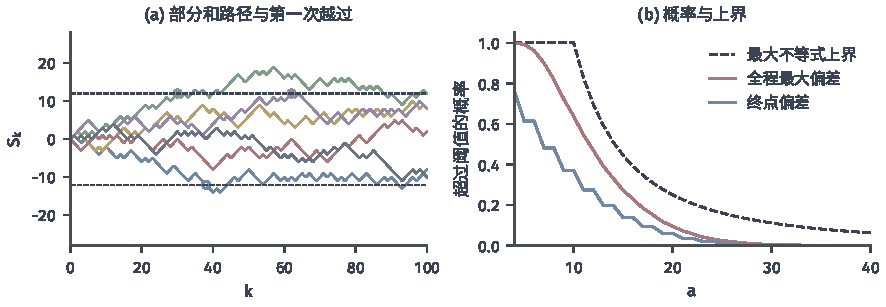
\includegraphics[width=150mm]{figures/02-abstract-mathematics/02-probability-spaces/matplotlib/conv-kolmogorov-maximal/figure.pdf}
  \caption{独立$\pm1$步长部分和的最大偏差，$n=100$。(a) 用固定随机种子画出的$6$条路径$S_k$，虚线为$\pm12$，空心圆标出各路径第一次满足$|S_k|\geq12$的位置；(b) $20000$次模拟中$\max_{k\leq100}|S_k|\geq a$（红）与$|S_{100}|\geq a$（蓝）的频率，虚线为最大不等式的上界$\min\{1,100/a^2\}$。终点曲线呈阶梯状，是因为$S_{100}$只取偶数值。}
  \label{fig:conv-kolmogorov-maximal}
\end{figure*}

\paragraph{按第一次越过的位置分解}
证明的想法是：把“曾经越过阈值”按\emph{第一次}越过的时刻分成互不相交的几种情形，在每种情形里，越过之后的增量与此前无关，平均起来不会把$S_n^2$拉小。

\begin{proof}
对$k=1,\ldots,n$，令
\[
  A_k=\bigl\{|S_k|\geq a,\ |S_j|<a\ \text{对所有}j<k\bigr\},
\]
即第一次越过阈值发生在时刻$k$。这些事件两两不交，并且$\bigcup_{k=1}^nA_k=\{\max_{k\leq n}|S_k|\geq a\}$。
记$R_k=S_n-S_k=\sum_{i=k+1}^nZ_i$为时刻$k$以后的增量。由于$\mathbb I_{A_k}\leq1$且两两不交，
\[
  \mathbb ES_n^2\geq\sum_{k=1}^n\mathbb E\bigl[S_n^2\,\mathbb I_{A_k}\bigr]
  =\sum_{k=1}^n\Bigl(\mathbb E\bigl[S_k^2\,\mathbb I_{A_k}\bigr]+2\,\mathbb E\bigl[S_k\mathbb I_{A_k}\cdot R_k\bigr]+\mathbb E\bigl[R_k^2\,\mathbb I_{A_k}\bigr]\Bigr).
\]
看中间的交叉项。$S_k\mathbb I_{A_k}$只依赖$Z_1,\ldots,Z_k$，$R_k$只依赖$Z_{k+1},\ldots,Z_n$；由第~\ref{chap:probability-models}章定理~\ref{thm:pmod-independence-grouping}，两组变量的函数相互独立。两者都有有限二阶矩，由Cauchy--Schwarz不等式（定理~\ref{thm:pmod-cauchy-schwarz}）其乘积可积，于是由定理~\ref{thm:pmod-product-expectation}，
\[
  \mathbb E\bigl[S_k\mathbb I_{A_k}\cdot R_k\bigr]=\mathbb E\bigl[S_k\mathbb I_{A_k}\bigr]\,\mathbb ER_k=0.
\]
第三项非负，舍去；在$A_k$上$S_k^2\geq a^2$。所以
\[
  \mathbb ES_n^2\geq\sum_{k=1}^n\mathbb E\bigl[S_k^2\,\mathbb I_{A_k}\bigr]\geq a^2\sum_{k=1}^n\mathbb P(A_k)=a^2\,\mathbb P\Bigl(\max_{1\leq k\leq n}|S_k|\geq a\Bigr).
\]
最后，$\mathbb ES_n^2=\operatorname{Var}(S_n)=\sum_i\operatorname{Var}(Z_i)$。
\end{proof}

整个证明只把一个事件分成了$n$个互不相交的事件；每个$A_k$由$Z_1,\ldots,Z_k$决定，而此后的增量$R_k$与它们独立且均值为零，这是交叉项消失的原因。
“第一次越过的时刻”是随机的，这一思想在卷三的停时与鞅理论中会得到系统发展，但这里不需要那些概念。

\subsection{方差可和条件下的级数收敛}

\paragraph{尾段的最大偏差}
现在考虑无穷多个独立、中心化的$Z_n$，问随机级数$\sum_nZ_n$何时几乎处处收敛。
\term{随机级数}（random series）收敛等价于部分和序列满足Cauchy条件，即足够晚以后任意两个部分和都很接近；这正是最大不等式能够控制的量。

\begin{theorem}[方差可和的独立级数]
\label{thm:conv-series}
设$Z_1,Z_2,\ldots$相互独立，$\mathbb EZ_n=0$，且$\sum_{n=1}^{\infty}\operatorname{Var}(Z_n)<\infty$。则$\sum_{n=1}^{\infty}Z_n$几乎处处收敛。
\end{theorem}

证明分两步。第一步把最大不等式用于从$m$开始的尾段。
对$m<j$，$S_k-S_m=\sum_{i=m+1}^kZ_i$（$m<k\leq j$）是独立中心化变量$Z_{m+1},\ldots,Z_j$的部分和，由定理~\ref{thm:conv-kolmogorov-maximal}，
\[
  \mathbb P\Bigl(\max_{m<k\leq j}|S_k-S_m|\geq\varepsilon\Bigr)\leq\frac1{\varepsilon^2}\sum_{i=m+1}^j\operatorname{Var}(Z_i)\leq\frac1{\varepsilon^2}\sum_{i>m}\operatorname{Var}(Z_i).
\]
若$\sup_{k>m}|S_k-S_m|>\varepsilon$，则存在某个$k$使$|S_k-S_m|>\varepsilon$，它属于$j=k$时左侧的事件。左侧事件随$j$递增，由概率的连续性，
\begin{equation}
  \mathbb P\Bigl(\sup_{k>m}|S_k-S_m|>\varepsilon\Bigr)\leq\frac1{\varepsilon^2}\sum_{i>m}\operatorname{Var}(Z_i).
  \label{eq:conv-tail-maximal}
\end{equation}
这个界同时控制了$m$以后\emph{所有}的部分和，而不只是某一个终点。

\paragraph{Cauchy条件与实数的完备性}
第二步把式~\eqref{eq:conv-tail-maximal}转化为Cauchy条件。

\begin{proof}[定理~\ref{thm:conv-series}的证明]
令$D_m=\sup_{k,l>m}|S_k-S_l|$，它衡量$m$以后部分和之间的最大差距。由三角不等式$|S_k-S_l|\leq|S_k-S_m|+|S_l-S_m|$，得$D_m\leq2\sup_{k>m}|S_k-S_m|$。
$D_m$随$m$递减，记其极限为$D=\lim_mD_m\in[0,\infty]$；对每个样本结果，部分和数列是Cauchy列当且仅当$D=0$。
对任意$\varepsilon>0$和任意$m$，$D\leq D_m$，所以由式~\eqref{eq:conv-tail-maximal}，
\[
  \mathbb P(D>2\varepsilon)\leq\mathbb P(D_m>2\varepsilon)\leq\mathbb P\Bigl(\sup_{k>m}|S_k-S_m|>\varepsilon\Bigr)\leq\frac1{\varepsilon^2}\sum_{i>m}\operatorname{Var}(Z_i).
\]
左侧与$m$无关，右侧是收敛级数的尾和，令$m\to\infty$得$\mathbb P(D>2\varepsilon)=0$。
取$\varepsilon=1/r$，$r=1,2,\ldots$，$\{D>0\}=\bigcup_r\{D>2/r\}$是可数个零概率事件之并，所以$D=0$几乎处处成立。
于是几乎每个样本结果上部分和都是实数的Cauchy列；由实数的完备性，它收敛。
\end{proof}

最后一步用的是每条样本路径上实数列的完备性：Cauchy数列必收敛。它与“平方可积随机变量构成完备空间”是不同的事实，后者属于第~\ref{part:function-spaces}部分，这里没有用到。
方差可和条件也蕴含$\mathbb E(S_n-S_m)^2=\sum_{i=m+1}^n\operatorname{Var}(Z_i)\to0$，即部分和的均方差距趋于零；但从均方差距到逐样本收敛，需要的正是最大不等式提供的全程控制。

\begin{example}[随机调和级数]
\label{ex:conv-random-harmonic}
设$\varepsilon_1,\varepsilon_2,\ldots$独立，各以概率$1/2$取$+1$和$-1$。
令$Z_n=\varepsilon_n/n$，则$\mathbb EZ_n=0$，$\sum_n\operatorname{Var}(Z_n)=\sum_n1/n^2=\pi^2/6<\infty$，由定理~\ref{thm:conv-series}，随机调和级数$\sum_n\varepsilon_n/n$几乎处处收敛。
普通的调和级数$\sum_n1/n$发散；随机符号使大部分项相互抵消，级数就收敛了。
更一般地，$\sum_n\varepsilon_n/n^{\alpha}$在$\alpha>1/2$时满足$\sum_nn^{-2\alpha}<\infty$，同样几乎处处收敛。
\end{example}

图~\ref{fig:conv-random-harmonic}左栏画出$\sum_{k\leq n}\varepsilon_k/k$的六条样本路径：每条路径在几百项以后几乎不再移动，但不同路径停在不同的值，极限本身是随机变量。
右栏是$\alpha=1/2$的临界情形$\sum_{k\leq n}\varepsilon_k/\sqrt k$，方差$\sum_{k\leq n}1/k$随$n$对数增长，定理~\ref{thm:conv-series}不适用；路径一直在游走，没有稳定下来。
事实上这个级数几乎处处发散，证明需要Kolmogorov三级数定理的必要性部分，本章不展开；由零一律（定理~\ref{thm:conv-zero-one}），它的收敛概率只能是$0$或$1$。

\begin{figure*}[htbp]
  \centering
  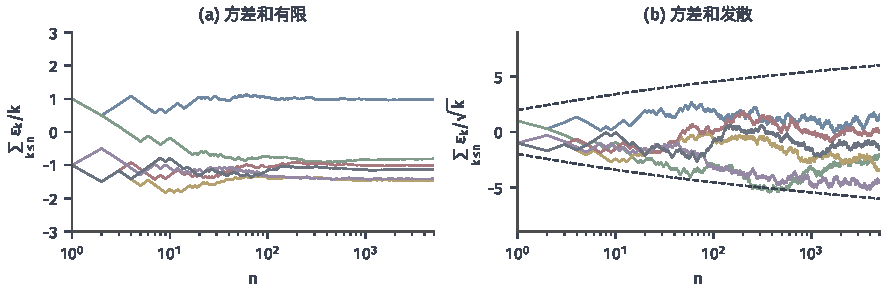
\includegraphics[width=150mm]{figures/02-abstract-mathematics/02-probability-spaces/matplotlib/conv-random-harmonic/figure.pdf}
  \caption{随机符号级数的部分和，$\varepsilon_k$独立且等概率取$\pm1$，横轴为对数刻度，用固定随机种子画出$6$条路径。(a) $\sum_{k\leq n}\varepsilon_k/k$，方差和为$\pi^2/6$，各路径在$n=5000$时分别停在约$-1.47$到$0.99$之间；(b) $\sum_{k\leq n}\varepsilon_k/\sqrt k$，虚线为$\pm2\bigl(\sum_{k\leq n}1/k\bigr)^{1/2}$，即两倍标准差。}
  \label{fig:conv-random-harmonic}
\end{figure*}

\subsection{由级数收敛得到平均值收敛}

\paragraph{Kronecker引理}
上一小节回答了级数何时收敛，而我们的最终目标是样本平均。
二者之间需要一个确定性的桥梁：若加权级数$\sum_nz_n/n$收敛，平均值$\frac1n\sum_{k=1}^nz_k$是否趋于零？
直觉是：$\sum z_n/n$收敛说明$z_n$的“累计贡献”增长得比$n$慢，所以除以$n$后消失。下面的\term{Kronecker引理}（Kronecker's lemma）用分部求和把这一直觉写成证明。

\begin{lemma}[Kronecker引理]
\label{lem:conv-kronecker}
设$z_1,z_2,\ldots$是实数，级数$\sum_{n=1}^{\infty}z_n/n$收敛。则
\[
  \lim_{n\to\infty}\frac1n\sum_{k=1}^nz_k=0.
\]
\end{lemma}

\begin{proof}
记$b_0=0$，$b_n=\sum_{k=1}^nz_k/k$，于是$z_k=k(b_k-b_{k-1})$，且$b_n\to b$为有限数。
用\term{Abel分部求和}（summation by parts）重新整理$\sum_{k=1}^nz_k$：
\[
  \sum_{k=1}^nk(b_k-b_{k-1})=\sum_{k=1}^nkb_k-\sum_{k=0}^{n-1}(k+1)b_k=nb_n-\sum_{k=1}^{n-1}b_k,
\]
最后一步把两个和中$k=1,\ldots,n-1$的项合并，$kb_k-(k+1)b_k=-b_k$，并用了$b_0=0$。两边除以$n$，
\begin{equation}
  \frac1n\sum_{k=1}^nz_k=b_n-\frac1n\sum_{k=1}^{n-1}b_k.
  \label{eq:conv-abel-identity}
\end{equation}
右侧第一项趋于$b$。第二项是$b_k$的\term{Cesàro平均}（Cesàro mean），也趋于$b$：对$\eta>0$取$N$使$k\geq N$时$|b_k-b|<\eta$，则当$n>N$时
\[
  \Bigl|\frac1n\sum_{k=1}^{n-1}b_k-b\Bigr|\leq\frac1n\sum_{k=1}^{N-1}|b_k-b|+\frac{n-N}{n}\,\eta+\frac{|b|}{n},
\]
右侧第一项和第三项的分子固定，随$n\to\infty$趋于$0$，所以上极限不超过$\eta$。
两项极限相同，相减得$0$。
\end{proof}

式~\eqref{eq:conv-abel-identity}是整个证明的核心：平均值等于加权部分和与它自身Cesàro平均的差，而一个收敛数列和它的Cesàro平均趋于同一极限。
图~\ref{fig:conv-kronecker}在随机调和级数的一条路径上画出了这三个量。
$b_n$在约$0.99$附近稳定下来，它的Cesàro平均以更平缓的方式追上它；两者之差就是$\varepsilon_k$的平均值，在$n=5000$时为$0.006$。

\begin{figure}[htbp]
  \centering
  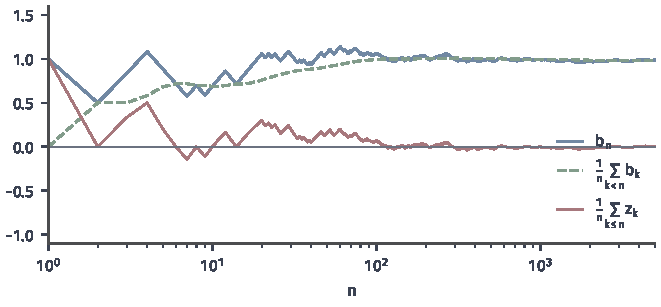
\includegraphics[width=112mm]{figures/02-abstract-mathematics/02-probability-spaces/matplotlib/conv-kronecker/figure.pdf}
  \caption{Kronecker引理中的恒等式~\eqref{eq:conv-abel-identity}，取$z_k=\varepsilon_k$为图~\ref{fig:conv-random-harmonic}(a)中第一条路径的随机符号，横轴为对数刻度。蓝线为$b_n=\sum_{k\leq n}z_k/k$，绿色虚线为其Cesàro平均$\frac1n\sum_{k<n}b_k$，红线为二者之差，即平均值$\frac1n\sum_{k\leq n}z_k$。}
  \label{fig:conv-kronecker}
\end{figure}

\begin{example}[确定性数列上的Kronecker引理]
\label{ex:conv-kronecker-deterministic}
取$z_k=(-1)^{k+1}\sqrt k$。级数$\sum_kz_k/k=\sum_k(-1)^{k+1}/\sqrt k$是交错级数，各项绝对值单调趋于零，所以收敛（其和约为$0.605$）。
由Kronecker引理，$\frac1n\sum_{k=1}^n(-1)^{k+1}\sqrt k\to0$；直接计算，$n=100$、$1000$、$10000$时这一平均值分别约为$-0.046$、$-0.015$、$-0.005$。
引理的逆命题不成立：$z_k=1/\ln(k+1)$满足$z_k\to0$，因而其Cesàro平均趋于$0$，但$\sum_k1/(k\ln(k+1))$发散。
\end{example}

\paragraph{逐个样本结果上的应用}
Kronecker引理是关于实数列的结论，用于随机变量时要逐个样本结果使用。
若存在概率为$1$的事件$E$，使每个$\omega\in E$上级数$\sum_nZ_n(\omega)/n$收敛，则对这些$\omega$都有$\frac1n\sum_{k=1}^nZ_k(\omega)\to0$，即$\frac1n\sum_{k=1}^nZ_k\xrightarrow{\mathrm{a.s.}}0$。
结合定理~\ref{thm:conv-series}，只需检验$Z_n/n$独立、中心化且$\sum_n\operatorname{Var}(Z_n)/n^2<\infty$。
这就是下一节的出发点。
引理还有一般的形式：若$0<a_n\uparrow\infty$且$\sum_nz_n/a_n$收敛，则$a_n^{-1}\sum_{k\leq n}z_k\to0$，证明方法相同；本章只用$a_n=n$的情形。

\section{样本平均的收敛}
\label{sec:conv-sample-means}

本节研究部分和按项数归一化后得到的样本平均$\bar X_n=\frac1n\sum_{k=1}^nX_k$。
我们回到章首的问题：卷一的弱大数律说$\bar X_n$偏离均值的概率趋于零，现在要证明更强的结论——几乎每条样本序列上$\bar X_n$都收敛到均值。
先说明为什么弱大数律的证明不能直接升级，再分两步证明：方差可和时直接用上一节的工具，只有一阶矩时用截断把问题化回方差可和的情形。

\subsection{从弱大数律到强大数律}

\paragraph{已有的弱大数律}
卷一已经证明：若$X_1,X_2,\ldots$独立同分布且$\mathbb E|X_1|<\infty$，则$\bar X_n\xrightarrow{\mathbb P}\mathbb EX_1$。
有限方差时那里用的是Chebyshev不等式；只有一阶矩时，那里先把每个观测在固定水平$M$处截断，用Markov不等式控制截断掉的尾部，再用Chebyshev控制有界部分。
本节不重复这些证明，而是讨论比它更强的结论。

\begin{definition}[强大数定律]
\label{def:conv-slln}
设随机变量列$(X_n)$的各项有相同的有限均值$\mu$。若$\bar X_n\xrightarrow{\mathrm{a.s.}}\mu$，称$(X_n)$满足\term{强大数定律}（strong law of large numbers），简称强大数律。
\end{definition}

“强”与“弱”的差别就是第~\ref{sec:conv-modes}节中几乎处处收敛与依概率收敛的差别。
由定理~\ref{thm:conv-implications}(1)，在相同条件下证明了强大数律，弱大数律就自动成立。
对章首的硬币问题，强大数律说的是：几乎每一次运行产生的频率序列，本身都收敛到$1/2$。

\paragraph{Chebyshev界为何不够}
设$X_n$独立同分布，方差$0<\sigma^2<\infty$，均值$\mu$。
Chebyshev不等式给出
\[
  \mathbb P(|\bar X_n-\mu|\geq\varepsilon)\leq\frac{\sigma^2}{n\varepsilon^2}.
\]
要用Borel--Cantelli引理得到几乎处处收敛，需要对每个$\varepsilon$这些概率可求和；但$\sum_n\sigma^2/(n\varepsilon^2)$是调和级数，发散。
所以不能把弱大数律的这一证明与Borel--Cantelli引理机械地连接起来。

图~\ref{fig:conv-chebyshev-nonsummable}以$\operatorname{Bernoulli}(1/2)$样本、$\varepsilon=0.1$为例做了比较。
Chebyshev上界是$\min\{1,25/n\}$；精确的误差概率由二项分布算出，$n=100$时约为$0.057$，$n=500$时约为$9\times10^{-6}$，下降远快于$1/n$。
右图中，精确概率的累计和到$n=2000$约为$26$且已停止增长，而上界的累计和约为$134$并按对数继续增长。
所以在这个例子里失效的是上界，不是事实本身：真实的误差概率是可求和的。
但只假设有限方差时，我们手中只有Chebyshev这样的二阶矩信息，必须找到不依赖指数小尾部的论证。

\begin{figure*}[htbp]
  \centering
  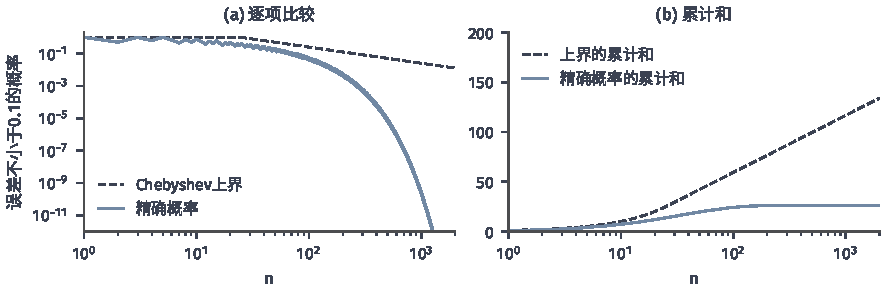
\includegraphics[width=150mm]{figures/02-abstract-mathematics/02-probability-spaces/matplotlib/conv-chebyshev-nonsummable/figure.pdf}
  \caption{$\operatorname{Bernoulli}(1/2)$样本平均的误差概率$\mathbb P(|\bar X_n-1/2|\geq0.1)$，横轴为对数刻度。(a) 精确值（由二项分布计算，蓝线）与Chebyshev上界$\min\{1,25/n\}$（虚线），纵轴为对数刻度；(b) 二者自$n=1$起的累计和，$n=2000$时分别约为$26.3$与$134.1$。}
  \label{fig:conv-chebyshev-nonsummable}
\end{figure*}

不过Chebyshev界并非毫无用处。
沿子列$n=m^2$，$\sum_m\sigma^2/(m^2\varepsilon^2)<\infty$，所以由Borel--Cantelli引理，$\bar X_{m^2}\xrightarrow{\mathrm{a.s.}}\mu$。
困难在于子列之间：$m^2$与$(m+1)^2$之间有$2m$项，需要控制$\bar X_n$在这一段中的全程波动。
这正是最大偏差的问题。第~\ref{sec:conv-partial-sums}节的最大不等式、级数收敛和Kronecker引理，提供了一条不经过子列、直接控制整条序列累计误差的路线。

\subsection{方差可和条件下的强大数律}

\paragraph{中心化后的加权级数}
把上一节的结论组合起来，先得到一个允许各项分布不同的版本。

\begin{theorem}[方差可和条件下的强大数律]
\label{thm:conv-slln-variance}
设$X_1,X_2,\ldots$相互独立，各有有限方差，且
\[
  \sum_{n=1}^{\infty}\frac{\operatorname{Var}(X_n)}{n^2}<\infty.
\]
则
\[
  \frac1n\sum_{k=1}^n\bigl(X_k-\mathbb EX_k\bigr)\xrightarrow{\mathrm{a.s.}}0.
\]
\end{theorem}

\begin{proof}
令$W_n=X_n-\mathbb EX_n$。变量$W_n/n$相互独立（各是$X_n$的函数），均值为零，方差$\operatorname{Var}(X_n)/n^2$可和。
由定理~\ref{thm:conv-series}，$\sum_nW_n/n$几乎处处收敛；在这个概率为$1$的事件上逐样本应用引理~\ref{lem:conv-kronecker}，得$\frac1n\sum_{k=1}^nW_k\to0$。
\end{proof}

这一结论不要求同分布，所得极限是减去各项期望之后的平均误差。
例如各批产品的合格率$p_n$不同，第$n$件是否合格记为$X_n\sim\operatorname{Bernoulli}(p_n)$，各件独立。
由于$\operatorname{Var}(X_n)=p_n(1-p_n)\leq1/4$，$\sum_n\operatorname{Var}(X_n)/n^2\leq\pi^2/24$，所以合格频率与平均合格率之差$\frac1n\sum_{k\leq n}(X_k-p_k)$几乎处处趋于零。
若$p_n$本身没有极限，合格频率也未必收敛，但它始终贴着$\frac1n\sum_{k\leq n}p_k$变化。

\paragraph{独立同分布且方差有限的情形}
独立同分布且方差$\sigma^2<\infty$时，$\sum_n\sigma^2/n^2<\infty$，定理~\ref{thm:conv-slln-variance}给出$\bar X_n\xrightarrow{\mathrm{a.s.}}\mu$。
同一条件下也有$\mathbb E(\bar X_n-\mu)^2=\sigma^2/n\to0$，即$\bar X_n\xrightarrow{L^2}\mu$。
两个结论都在“方差有限”下成立，但依据不同：均方收敛只需计算一个方差，几乎处处收敛还需要最大不等式对全程波动的控制。
二者互不蕴含，这在第~\ref{sec:conv-modes}节的反例中已经看到。

图~\ref{fig:conv-slln-paths}(a)画出均值为$1$的指数分布样本的五条平均值路径，它们在$n=10^5$时与$1$的距离都不超过$0.005$。
这一证明还没有覆盖只有有限一阶矩的样本：例如指数为$1.5$的Pareto分布有均值，方差却是无穷大，定理~\ref{thm:conv-slln-variance}的条件不满足。

\subsection{有限一阶矩条件下的强大数律}

\paragraph{定理与证明路线}
现在陈述本章的主要结论。

\begin{theorem}[强大数律]
\label{thm:conv-slln}
设$X_1,X_2,\ldots$独立同分布，$\mathbb E|X_1|<\infty$，$\mu=\mathbb EX_1$。则$\bar X_n\xrightarrow{\mathrm{a.s.}}\mu$。
\end{theorem}

条件中没有方差，所以不能直接用定理~\ref{thm:conv-slln-variance}。
办法与卷一的弱大数律类似，也是截断，但截断水平不再固定，而是随项数增长：令
\[
  Y_n=X_n\,\mathbb I_{\{|X_n|\leq n\}}.
\]
随$n$增大的截断水平带来三方面的结果，图~\ref{fig:conv-slln-roadmap}把它们和上一节的工具画在一起：截断改变的项只有有限个；截断项虽不同分布，却满足方差可和条件；截断项的期望仍趋于$\mu$。
下面三段依次证明这三点。

\begin{figure*}[htbp]
  \centering
  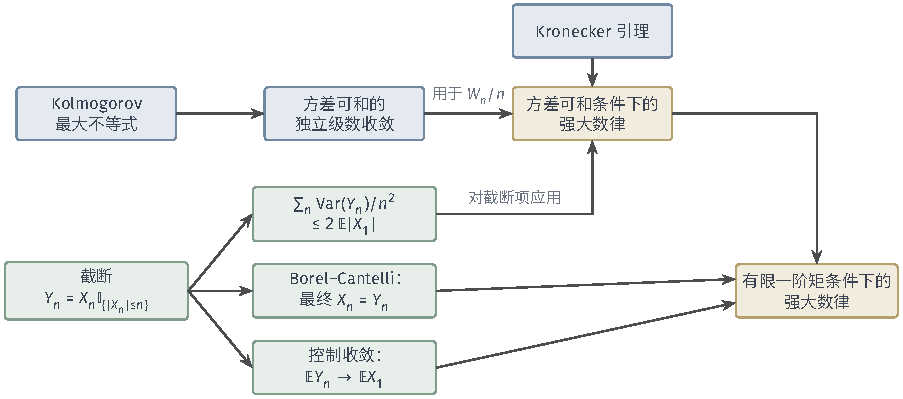
\includegraphics[width=153mm]{figures/02-abstract-mathematics/02-probability-spaces/tikz/conv-slln-roadmap/figure.pdf}
  \caption{强大数律的证明路线。蓝框是第~\ref{sec:conv-partial-sums}节的工具，绿框是截断$Y_n=X_n\mathbb I_{\{|X_n|\leq n\}}$带来的三步推导，黄框是两个层次的强大数律；箭头表示推导所用的依赖关系，$W_n=X_n-\mathbb EX_n$。}
  \label{fig:conv-slln-roadmap}
\end{figure*}

\paragraph{截断项与原序列最终一致}
由同分布，$\mathbb P(|X_n|>n)=\mathbb P(|X_1|>n)$。
对$t\in[n-1,n]$有$\mathbb P(|X_1|>n)\leq\mathbb P(|X_1|>t)$，所以
\[
  \begin{aligned}
  \sum_{n=1}^{\infty}\mathbb P(|X_n|>n)
  &\leq\sum_{n=1}^{\infty}\int_{n-1}^n\mathbb P(|X_1|>t)\,dt\\
  &=\int_0^{\infty}\mathbb P(|X_1|>t)\,dt=\mathbb E|X_1|<\infty.
  \end{aligned}
\]
最后一个等号是把$|X_1|=\int_0^{\infty}\mathbb I_{\{t<|X_1|\}}\,dt$代入期望，再对非负被积函数交换积分次序（定理~\ref{thm:analysis-tonelli-fubini}的Tonelli部分）。
由Borel--Cantelli引理第一部分，几乎必然只有有限个$n$满足$|X_n|>n$，即存在依赖于$\omega$的$N$，使$n\geq N$时$X_n=Y_n$。
于是$\sum_{k=1}^n(X_k-Y_k)$从某项起不再变化，是一个固定的有限数，除以$n$后趋于$0$：
\[
  \frac1n\sum_{k=1}^n(X_k-Y_k)\xrightarrow{\mathrm{a.s.}}0.
\]

图~\ref{fig:conv-truncation}以指数为$1.5$的Pareto分布为例。
它满足$\mathbb P(X_1>t)=t^{-1.5}$（$t\geq1$），均值为$3$，方差无穷大；被截断的项数的期望为$\sum_nn^{-1.5}\approx2.61$。
在所画的样本中，只有$n=1,3,11,93$四项超过了截断水平，此后再也没有；右图显示两种样本平均之差在$n=93$以后严格按“常数$/n$”衰减。

\begin{figure*}[htbp]
  \centering
  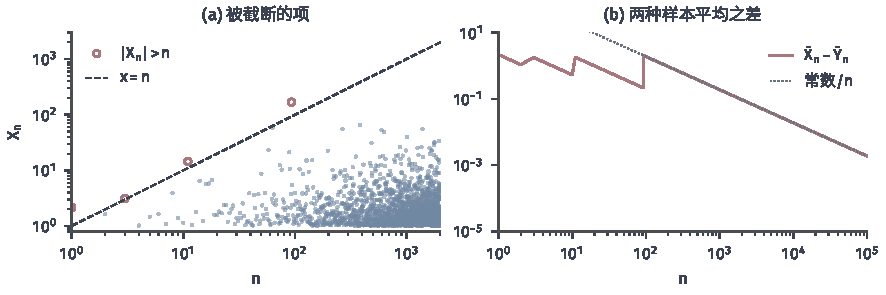
\includegraphics[width=150mm]{figures/02-abstract-mathematics/02-probability-spaces/matplotlib/conv-truncation/figure.pdf}
  \caption{截断$Y_n=X_n\mathbb I_{\{|X_n|\leq n\}}$与原序列的最终一致，$X_n$独立服从指数为$1.5$、下界为$1$的Pareto分布，固定随机种子。(a) 前$2000$个观测（双对数坐标），虚线为截断水平$x=n$，红圈为被截断的项，本样本中为$n=1,3,11,93$；(b) $\bar X_n-\bar Y_n$，$n\leq10^5$，点线为被截断部分的总和除以$n$。}
  \label{fig:conv-truncation}
\end{figure*}

\paragraph{截断项的方差可和}
截断项$Y_n$是独立的$X_n$各自的函数，所以仍相互独立，但截断水平随$n$变化，它们一般不再同分布。
每个$Y_n$以$n$为界，方差有限，且
\[
  \operatorname{Var}(Y_n)\leq\mathbb EY_n^2=\mathbb E\bigl[X_1^2\,\mathbb I_{\{|X_1|\leq n\}}\bigr],
\]
这里再次用了同分布。对非负项交换求和与期望（单调收敛定理），
\[
  \sum_{n=1}^{\infty}\frac{\operatorname{Var}(Y_n)}{n^2}\leq\mathbb E\Bigl[X_1^2\sum_{n\geq1,\ n\geq|X_1|}\frac1{n^2}\Bigr].
\]
现在估计内层的尾和。对正整数$m$，$\sum_{n\geq m}n^{-2}\leq m^{-2}+\int_m^{\infty}t^{-2}\,dt=m^{-2}+m^{-1}\leq2/m$。
若$|X_1|\geq1$，取$m=\lceil|X_1|\rceil\geq|X_1|$，内层和不超过$2/|X_1|$，乘以$X_1^2$后不超过$2|X_1|$；
若$|X_1|<1$，内层和是$\sum_{n\geq1}n^{-2}<2$，而$X_1^2\leq|X_1|$，乘积也不超过$2|X_1|$。
两种情形合起来得到
\[
  \sum_{n=1}^{\infty}\frac{\operatorname{Var}(Y_n)}{n^2}\leq2\,\mathbb E|X_1|<\infty.
\]
这是截断水平取$n$的关键：大的$|X_1|$只在$n\geq|X_1|$的项中出现，而这些项的权重$1/n^2$之和约为$1/|X_1|$，恰好把二阶量$X_1^2$降为一阶量$|X_1|$。
由定理~\ref{thm:conv-slln-variance}，
\[
  \frac1n\sum_{k=1}^n\bigl(Y_k-\mathbb EY_k\bigr)\xrightarrow{\mathrm{a.s.}}0.
\]

\paragraph{均值的恢复与三步合并}
还需说明截断项的期望趋于$\mu$。
由同分布，$\mathbb EY_n=\mathbb E[X_1\,\mathbb I_{\{|X_1|\leq n\}}]$。被积函数逐点趋于$X_1$，且以可积的$|X_1|$为界，由控制收敛定理，$\mathbb EY_n\to\mathbb EX_1=\mu$。
一个收敛数列的Cesàro平均趋于同一极限（这一点已在引理~\ref{lem:conv-kronecker}的证明中说明），所以$\frac1n\sum_{k=1}^n\mathbb EY_k\to\mu$。

把三步合在一起：
\[
  \bar X_n-\mu=\frac1n\sum_{k=1}^n(X_k-Y_k)+\frac1n\sum_{k=1}^n\bigl(Y_k-\mathbb EY_k\bigr)+\Bigl(\frac1n\sum_{k=1}^n\mathbb EY_k-\mu\Bigr).
\]
第一项由Borel--Cantelli引理几乎处处趋于$0$，第二项由方差可和的强大数律几乎处处趋于$0$，第三项是确定的数列，趋于$0$。
三个概率为$1$的事件之交仍有概率$1$，在其上$\bar X_n\to\mu$。定理~\ref{thm:conv-slln}得证。

一阶矩条件不能再去掉。
若$X_n$独立同分布而$\mathbb E|X_1|=\infty$，反方向的比较（对$t\in[n,n+1]$有$\mathbb P(|X_1|>n)\geq\mathbb P(|X_1|>t)$）给出$\sum_n\mathbb P(|X_n|>n)\geq\int_1^{\infty}\mathbb P(|X_1|>t)\,dt\geq\mathbb E|X_1|-1=\infty$；事件$\{|X_n|>n\}$相互独立，由Borel--Cantelli引理第二部分，几乎必然有无穷多个$n$满足$|X_n|>n$。
另一方面$X_n/n=\bar X_n-\frac{n-1}{n}\bar X_{n-1}$，若$\bar X_n$收敛到有限极限，右侧趋于$0$，与$|X_n|/n>1$无穷多次发生矛盾。
所以这时$\bar X_n$几乎必然不收敛到任何有限数。

图~\ref{fig:conv-slln-paths}对照了三种情形。
指数分布有有限方差，路径很快稳定；指数为$1.5$的Pareto分布只有一阶矩，路径时常被一个大观测拉开，但最终仍回到均值$3$附近，$n=10^5$时五条路径在$2.91$到$2.96$之间，收敛明显更慢；指数为$0.8$的Pareto分布没有均值，平均值被越来越大的观测不断推高，五条路径在$n=10^5$时散布在$60$到$980$之间。

\begin{figure*}[htbp]
  \centering
  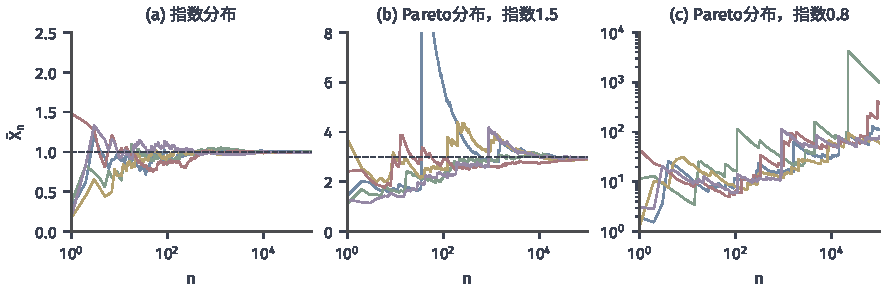
\includegraphics[width=150mm]{figures/02-abstract-mathematics/02-probability-spaces/matplotlib/conv-slln-paths/figure.pdf}
  \caption{独立同分布样本平均$\bar X_n$的路径，每个面板用固定随机种子画出$5$条，横轴为对数刻度，$n\leq10^5$。(a) 均值为$1$的指数分布，有有限方差；(b) 指数为$1.5$、下界为$1$的Pareto分布，均值为$3$（虚线），方差无穷；(c) 指数为$0.8$的Pareto分布，均值无穷，纵轴也为对数刻度。}
  \label{fig:conv-slln-paths}
\end{figure*}

\paragraph{函数的样本平均}
强大数律对任何满足矩条件的函数都成立。
设$g$可测且$\mathbb E|g(X_1)|<\infty$；$g(X_1),g(X_2),\ldots$仍独立同分布，把定理~\ref{thm:conv-slln}用于它们，得
\[
  \frac1n\sum_{k=1}^ng(X_k)\xrightarrow{\mathrm{a.s.}}\mathbb Eg(X_1).
\]
取$g=\mathbb I_B$，得到事件$\{X_k\in B\}$的经验频率几乎必然收敛到$P_{X_1}(B)$，这回答了章首的硬币问题。
取$g(x)=x^r$，$r$为正整数且$\mathbb E|X_1|^r<\infty$，得到样本$r$阶矩的收敛。
记$F$为$X_1$的分布函数，固定$x$并取$g=\mathbb I_{(-\infty,x]}$，经验分布函数在点$x$处几乎必然收敛到$F(x)$。

强大数律是渐近结论。
它不给出固定样本量下误差超过阈值的概率，也不给出收敛速度：图~\ref{fig:conv-slln-paths}(b)的样本平均同样收敛，但速度明显比(a)慢，这是定理本身看不出来的。
误差放大$\sqrt n$倍以后的分布规律由下一章（第~\ref{chap:weak-convergence-limit-theorems}章）的中心极限定理描述。
对一整族函数同时成立的收敛，例如经验分布函数在所有$x$上的一致收敛，属于\BookPartRef{part:inference-and-causal-identification}{卷四“推断与因果识别”部分}；观测相互依赖、平均沿时间进行的情形属于\BookPartRef{part:dynamical-systems-control-decision-and-games}{卷三“过程与轨迹演化”部分}。

\section{本章小结}
\label{sec:conv-summary}

\paragraph{三种收敛与两种失效}
章首问了随机误差以什么意义趋于零。
几乎处处收敛看每个样本结果的整条数列，依概率收敛看每个时刻坏事件的概率，$p$阶平均收敛看误差幅度的平均；几乎处处收敛和$p$阶平均收敛都蕴含依概率收敛，高阶平均收敛蕴含低阶平均收敛。
逆命题的失效有两种典型机制：二进区间扫描中坏事件越来越小却反复发生，所以依概率收敛和平均收敛都推不出几乎处处收敛；尖峰中坏事件只发生有限次却幅度极大，所以几乎处处收敛推不出平均收敛。
两种失效分别由两个工具修补。
Borel--Cantelli引理把“坏事件概率可求和”转化为“坏事件只发生有限次”，由此得到子列判据：依概率收敛恰好等价于每个子列都有几乎处处收敛的进一步子列。它使控制收敛这类逐点定理可以用于依概率收敛。
一致可积要求同一个阈值控制全族的尾部积分，它排除了稀有大值对平均误差的持续贡献；在依概率收敛下，它恰好等价于一阶平均收敛，期望的收敛随之而来，并可进一步传入固定信息下的条件期望。

\paragraph{强大数律的证明链}
章首还问了独立样本的平均何时沿几乎每条样本序列趋于总体均值。
Chebyshev界不可求和，说明单靠逐个时刻的二阶矩控制不够，需要控制整个过程的累计误差。
Kolmogorov最大不等式按第一次越过阈值的位置分解事件，使全程最大偏差与终点偏差共享同一个方差上界；由此，方差可和的独立级数几乎处处收敛；Kronecker引理再把加权级数的收敛化为平均值的收敛，得到方差可和条件下的强大数律。
只有一阶矩时，随项数增长的截断同时做到三件事：只改变有限多项，使截断项的方差满足可和条件，并保持期望的极限。
整条证明只用到有限事件分解、独立性、积分收敛定理和实数的完备性，不需要鞅或函数空间。

本章始终在同一个概率空间上比较$X_n$与$X$，误差$X_n-X$对每个样本结果都有意义。
下一章放弃这一前提，只比较分布：随机变量可以定义在不同的空间上，我们问它们的分布是否趋于某个极限分布，何时存在收敛的子列，以及如何识别并传递分布的极限。
